\documentclass[11pt]{article}
\usepackage[notes]{yalatex}
% \addbibresource{references.bib}   % uncomment for citations

% Unnumbered chapter titles for the five parts of the course. Section numbers
% keep running across chapters, and each chapter gets an unnumbered entry in
% the table of contents (and a top-level PDF bookmark).
% Spacing: change these two lengths. 0pt means "as tight as possible".
\newlength{\chapterspaceabove}\setlength{\chapterspaceabove}{1em}
\newlength{\chapterspacebelow}\setlength{\chapterspacebelow}{1em}
\newcommand{\notechapter}[1]{%
  \par
  \phantomsection
  \addcontentsline{toc}{part}{#1}%
  % The space above is built into the title line (an invisible strut) instead
  % of a \vspace, because \vspace at the top of a page is either thrown away
  % or adds extra hidden space.
  {\centering\normalfont\Huge\bfseries
    \rule{0pt}{\dimexpr\fontcharht\font`d+\chapterspaceabove\relax}#1\par}%
  \vspace{0.4em}%
  \noindent\rule{\textwidth}{0.8pt}\par% underline
  \nobreak\nointerlineskip
  % An invisible strut of the requested height after the rule. (A \vspace here
  % would be swallowed by the section heading's own space above.)
  {\parskip=0pt \noindent\rule{0pt}{\chapterspacebelow}\par}%
  \nobreak
}

\title{MATH407: Advanced Number Theory}
\author{Notes by Yuval Amit}
\date{Instructor: Niranjan Ramachandran \\ Fall 2025}

\begin{document}
\maketitle

\tableofcontents
\newpage

\notechapter{Finite Fields}
% !TEX root = ../math407-notes.tex
% Transcribed from handwritten notes (1.1 Generalities, 1.2 Equations Over a
% Finite Field, 1.3 Quadratic Reciprocity).

\section{Preliminaries}

Let $K$ be a field. Then, $(K^\times, \cdot)$ is an abelian group. We have a homomorphism $\Z \to K$ by $1 \mapsto 1$, and its image $\Img(\Z) \subset K$ is a domain. So, either
$$\Z \hookrightarrow K \quad (\Char K = 0), \quad \text{or} \quad \Z \twoheadrightarrow \Z/p\Z \hookrightarrow K \quad (\Char K = p).$$
In the first case, $\Z \hookrightarrow K$ is equivalent to $\Q \hookrightarrow K$.

\begin{notebox*}[Observation]
    If $K$ has characteristic $p$, then there exists a ring homomorphism $\phi : K \to K$ given by $\phi(x) = x^p$, since
    $$\phi(x+y) = (x+y)^p = x^p + y^p + 0.$$
    Since $K$ is a field, $\phi$ must be injective, since the kernel must be trivial.
\end{notebox*}

\begin{defn}
    Let $K$ have characteristic $p$. Then, $K$ is \textbf{perfect} if $\phi : K \to K$ is an automorphism.
\end{defn}

\begin{ex}
    \begin{enumerate}
        \item An algebraically closed field $K = \bar K$ of characteristic $p$.
        \item $\F_p = \Z/p\Z$.
    \end{enumerate}
\end{ex}

\begin{defn}
    The map $\phi$ is called the \textbf{Frobenius map}.
\end{defn}

\begin{thm}
    Let $R$ be a finite domain. Then, $R$ must be a field.
\end{thm}

\begin{proof}
    For $x \neq 0$, the map $\phi_x : R \to R$ given by $y \mapsto xy$ is a bijection, so $\phi_x(y) = 1$ has a solution.
\end{proof}

\begin{thm}
    Let $K$ be a finite field.
    \begin{enumerate}[(1)]
        \item $\Char K = p > 0$, and $|K| = p^f$.
        \item Let $q = p^f$, $f \geq 1$, and let $\Omega$ be an algebraically closed field of characteristic $p$. Then, there exists a unique subfield of $\Omega$ of order $q$, denoted
        $$\F_q = \{\text{roots of } x^q - x \text{ in } \Omega\}.$$
        \item Any finite field of order $q$ is isomorphic to $\F_q$.
    \end{enumerate}
\end{thm}

\begin{proof}
    \hfill
    \begin{enumerate}[(1)]
        \item $K$ has characteristic $p$ because $\Q \not\hookrightarrow K$, hence $\Z/p\Z \hookrightarrow K$. So, $K$ is a vector space over $\Z/p\Z$, and $\dim(K)$ over $\F_p$ is finite. The degree of the extension is the same as the dimension of the vector space, so $|K| = p^f$, where $f$ is the degree.
        \item Let $\Omega$ be an algebraically closed field of characteristic $p$, and let $\phi : \Omega \to \Omega$ be given by $\phi(x) = x^q$. Then, $\phi$ is injective, and surjective by algebraic closure, hence is an automorphism. For any automorphism $T : E \to E$ of a field, the set
        $$F = \{x \in E \mid T(x) = x\} \subset E$$
        is a subfield. Let $\F_q$ be the set of elements fixed by $\phi$. All of its elements are roots of $x^q - x$, which has at most $q$ roots. Note that
        $$\frac{d}{dx}(x^q - x) = qx^{q-1} - 1 = -1 \neq 0,$$
        hence $x^q - x$ has no repeated roots. That is, $|\F_q| = q$.
    \end{enumerate}
\end{proof}

\begin{lem}
    $\F_{p^e} \subset \F_{p^f} \iff e \mid f$.
\end{lem}

\begin{proof}
    This follows by degree considerations.
\end{proof}

\begin{proof}[Proof of (3)]
    Given $K$ with $|K| = q$, there exists an algebraically closed field $\Omega$ containing $K$. For example, we could take $\Omega = \bar K$. Then, $\Omega$ has characteristic $p$. Let
    $$\F_q = \{a \in \Omega : a^q = a\} \subset \Omega.$$
    We want to show that $K = \F_q$. We have $a^q - a = a(a^{q-1} - 1)$. Let $a \in K \setminus \{0\}$. Then, $a \in K^\times$ and $|K^\times| = q - 1$, hence $a^{q-1} = 1$, so $a \in \F_q$. Also, $0 \in \F_q$, so $K \subseteq \F_q$. However, $|K| = |\F_q|$, hence $K = \F_q$.
\end{proof}

\begin{ex}
    \begin{enumerate}
        \item $\F_{3^2} \cong \F_3[x]/(x^2+1)$.
        \item More generally, $\F_p[x]/(x^2+1) = \F_{p^2} \iff p \equiv 3 \pmod 4$.
        \item $\F_{3^3} \cong \F_3[x]/(x^3+2x+1)$.
    \end{enumerate}
\end{ex}

\begin{notebox*}[Recall]
    $(\Z,+)$ has no non-zero elements of finite order.
\end{notebox*}

\begin{defn}
    For $G$ abelian, let $G_t = \{g \in G : |g| < \infty\}$, called the \textbf{torsion} of $G$.
\end{defn}

\begin{ex}
    $\Q/\Z$ is a torsion group.
\end{ex}

\begin{defn}
    Let $A$ be an abelian group. $A$ is \textbf{divisible} if for every map $A \to A$ given by $a \mapsto na$ with $n \in \Z \setminus \{0\}$ (where $na = a + \overset{n}{\cdots} + a$), the map is surjective. Note that these maps are always homomorphisms.
\end{defn}

\begin{ex}
    \begin{enumerate}
        \item $(\Z,+)$ is not divisible.
        \item $(\Q,+)$ is divisible.
        \item $\Q/\Z$ is divisible.
    \end{enumerate}
\end{ex}

\begin{defn}
    $A$ is \textbf{uniquely divisible} if all of those maps are automorphisms.
\end{defn}

\begin{ex}
    Consider the torsion of $(K^\times, \times)$ for the following fields $K$:
    \begin{center}
        \begin{tabular}{c|c}
            $K$ & Torsion of $K^\times$ \\ \hline
            $\Q$ & $\{\pm 1\}$ \\
            $\R$ & $\{\pm 1\}$ \\
            $\C$ & $\{\text{roots of unity}\} \cong \Q/\Z$ \\
            $\bar \Q$ & $\Q/\Z$
        \end{tabular}
    \end{center}
\end{ex}

\begin{thm}
    $(\F_q)^\times$ is cyclic. For $q = p$, this is equivalent to there being a primitive root modulo $p$.
\end{thm}

\begin{proof}
    \begin{notebox*}[Fact]
        Let $C_n = \angles{\sigma}$ be the cyclic group of order $n$, so $|\sigma| = n$. Then, $|\sigma^k| = \frac{n}{(k,n)}$. So,
        $$\#\{x \in C_n : |x| = n\} = \varphi(n).$$
        That is, $C_n$ has exactly $\varphi(n)$ generators.
    \end{notebox*}

    \begin{lem}
        Let $n \in \N$. Then, $n = \sum_{d \mid n} \varphi(d)$.
    \end{lem}

    \begin{proof}
        Let $\Phi_d = \{\text{elements of order } d \text{ in } C_n\}$. Then,
        $$C_n = \bigsqcup_{d \mid n} \Phi_d \implies \# C_n = \sum_{d \mid n} \# \Phi_d = \sum_{d \mid n} \varphi(d).$$
    \end{proof}

    \begin{lem}[Recognition of Finite Cyclic Groups]
        Let $H$ be finite and abelian, with $\# H = n$. Suppose that for all $d \mid n$, we have $\#\{a \in H : a^d = 1\} \leq d$. Then, $H \cong C_n$.
    \end{lem}

    \begin{proof}
        Let $d \mid n$, and let $H_d = \{a \in H : a^d = 1\}$. If there exists $x \in H$ of order $d$, then $\angles{x}$ has size $d$, and all elements $y \in \angles{x}$ satisfy $y^d = 1$. So, any $z \in H$ with $z^d = 1$ must be in $\angles{x}$. That is, $H_d \leq \angles{x}$. Hence, all elements of order $d$ are generators of $\angles{x} \leq H$, so there are exactly $\varphi(d)$ elements of order $d$ in $H$. So, if $d \mid n$, the number of elements of order $d$ in $H$ is either $0$ or $\varphi(d)$. Since $\# H = \sum_{d \mid n} \varphi(d)$, by counting we need an element of every order. In particular, $H$ has an element of order $n$.
    \end{proof}

    Now, let $H = (\F_q)^\times$, $n = q - 1$, and $H_d = \{a \in \F_q^\times : a^d = 1\}$. That is, $H_d = \{\text{roots of } x^d - 1 = 0\}$, and $x^d - 1$ has at most $d$ roots. So, $\# H_d \leq d$, hence $H$ is cyclic.
\end{proof}

\begin{notebox*}
    With the same argument, for any field $K$, any finite subgroup $H \leq K^\times$ is cyclic.
\end{notebox*}

\begin{ex}
    In $\F_5[x]$, we have $x^2 + 1 = (x+2)(x-2)$, so $\F_5[x]/(x^2+1) = \F_5[x]/(x+2)(x-2)$. Note that we have
    \[\begin{tikzcd}
        {\F_5[x]} && {\F_5[x]/(x+2)} \\
        \\
        {\F_5[x]/(x^2+1)}
        \arrow[two heads, from=1-1, to=1-3]
        \arrow[two heads, from=1-1, to=3-1]
        \arrow["{\exists}"', dashed, from=3-1, to=1-3]
    \end{tikzcd}\]
    where the dashed map exists because $x^2 + 1 \mapsto 0$. So, we get maps
    $$\F_5[x]/(x^2+1) \to \F_5[x]/(x+2) \cong \F_5, \qquad \F_5[x]/(x^2+1) \to \F_5[x]/(x-2) \cong \F_5,$$
    which combine to give $\F_5[x]/(x^2+1) \to \F_5 \times \F_5$.
\end{ex}

\section{Equations Over a Finite Field}

We look at equations over finite fields, and search for solutions.

\begin{defn}
    Let $g(x_1,\dots,x_n) \in \Z[x_1,\dots,x_n]$. The \textbf{solution set} of $g$ is
    $$V(g) = \{(a_1,\dots,a_n) \in \Z^n \mid g(a_1,\dots,a_n) = 0\}.$$
\end{defn}

\begin{ex}
    Let $f(x) = x^2 + 1$. If $f(a) = 0$, then $f(a) \equiv 0 \pmod p$ for all $p$. That is, $f$ has a root in $\F_p$. Let
    $$V_p(f) = \{\bar a \in \F_p : f(\bar a) = 0\}.$$
    If we can show $V_p(f)$ is empty for some prime $p$, then $V(f)$ is empty. Indeed, $V_3(f) = \emptyset$, hence $V(f) = \emptyset$.
\end{ex}

\begin{ex}
    Let $V(h) = \{(a,b,c) \mid a^5 + b^5 + c^5 = 0\}$. Does $V_p(h)$ non-empty imply $V(h)$ non-empty? \textbf{No.}
\end{ex}

\begin{notebox*}[Questions]
    \begin{enumerate}[(1)]
        \item Is every element of $\F_q$ a sum of $2$ squares? That is, does $x^2 + y^2 - a$ have a root for all $a \in \F_q$?
        \item Let $g(x,y,z) = 3x^2 + 5y^2 + 7z^2$, and let $a_p = |V_p(g)|$ be the number of solutions of $g$ in $\F_p$. What can we say about $a_p$? Is $\lim_{p \to \infty} a_p = \infty$, or is it bounded?
    \end{enumerate}
\end{notebox*}

\subsection{The Chevalley-Warning Theorem}

\begin{thm}[Chevalley-Warning Theorem][label=thm:chevalley-warning]
    Let $K = \F_q$ be a finite field, $R = K[x_1,\dots,x_n]$, and $f_1,\dots,f_r \in R$. Let $d = \deg f_1 + \cdots + \deg f_r$, and
    $$V = \{(a_1,\dots,a_n) \in K^n : f_j(a_1,\dots,a_n) = 0 \text{ for all } 1 \leq j \leq r\}.$$
    If $d < n$, then $\# V \equiv 0 \pmod p$.
\end{thm}

\begin{cor}
    Suppose in addition that $f_1,\dots,f_r$ have no constant term. Then, $V$ is non-empty because of the zero solution, hence $\# V \geq p$.
\end{cor}

\begin{cor}
    Let $f(x,y,z) = ax^2 + by^2 + cz^2 + dxy + exz + gyz$ be a quadratic form. Observe that $f(\lambda x, \lambda y, \lambda z) = \lambda^2 f(x,y,z)$. Since $f(0,0,0) = 0$, $f$ has a non-trivial solution in $\F_q$ as well.
\end{cor}

We can use this to answer question (1). Fix $a \in \F_q$, and consider $g(x,y,z) = x^2 + y^2 - az^2$. The theorem also answers question (2).

We can prove Chevalley-Warning with power sums.

\begin{ex}
    Let $K = \F_{11} = \{0,\dots,10\}$. For $m \geq 0$, let $f(x) = x^m$, and let $S_m = \sum_{a \in \F_{11}} a^m$. Note that
    $$S_0 = 0 \ (\text{taking } 0^0 = 1), \qquad S_1 = 0, \qquad S_{10} = 0 + 1 + \cdots + 1 = -1.$$
    What are $S_2$ and $S_3$?
\end{ex}

\begin{notebox*}[Observe]
    For a group $G$ and $g_0 \in G$, the map $g \mapsto g_0 g$ is a bijection.
\end{notebox*}

\begin{lem}[][label=lem:power-sums]
    Let $K = \F_q$ have characteristic $p$, with $q = p^f$. Let $S_m = \sum_{a \in K} a^m$, and more generally, if $f(x) = x^m$, let $S(f) = \sum_{a \in K} f(a)$. Then,
    \begin{enumerate}[(1)]
        \item $S_0 = 0$.
        \item If $m \geq 1$ and $q - 1 \mid m$, then $S_m = -1$.
        \item If $m \geq 1$ and $q - 1 \nmid m$, then $S_m = 0$.
    \end{enumerate}
\end{lem}

\begin{proof}
    \hfill
    \begin{enumerate}[(1)]
        \item $m = 0$ is clear.
        \item Suppose $q - 1 \mid m$. Then, for $a \in \F_q$, $a = 0 \implies a^m = 0$. Also, $a \neq 0 \implies a^m = 1$, since $\# \F_q^\times = q - 1$. So, $S_m = 0 + 1 + 1 + \cdots + 1 = -1$.
        \item Suppose $q - 1 \nmid m$. Then, there exists $y \neq 0$ in $K$ such that $y^m \neq 1$, because $K^\times$ is cyclic. Now, consider the map $K^\times \to K^\times$ given by $a \mapsto ay$, which is a bijection. Then,
        $$S_m = \sum_{a \in K^\times} a^m = \sum_{a \in K^\times} (ay)^m = y^m \sum_{a \in K^\times} a^m = y^m S_m.$$
        Thus, $(1 - y^m) S_m = 0$, and $1 - y^m \neq 0$, hence $S_m = 0$.
    \end{enumerate}
\end{proof}

\begin{lem}[][label=lem:monomial-sum]
    Let $g(x_1,\dots,x_n) \in R$ be a monomial, i.e. $g = x_1^{e_1} \cdots x_n^{e_n}$, and suppose $\sum e_i < (q-1)n$. As $g$ is a function $K^n \to K$, we can consider
    $$S(g) = \sum_{(a_1,\dots,a_n) \in K^n} g(a_1,\dots,a_n).$$
    Then, $S(g) = 0 \in K$.
\end{lem}

\begin{proof}
    By assumption, there exists $i$ with $e_i < q - 1$. Without loss of generality, suppose $i = 1$. Then,
    $$S(g) = \sum a_1^{e_1} \cdots a_n^{e_n} = \sum_{a_2,\dots,a_n} a_2^{e_2} \cdots a_n^{e_n} \paren{\sum_{a_1 \in K} a_1^{e_1}},$$
    but that last factor is $0$ by \Cref{lem:power-sums}, because $e_1 = 0$ or $q - 1 \nmid e_1$.
\end{proof}

\begin{ex}
    Let $W \subset \R$. The \textbf{characteristic function} of $W$ is
    $$\chi_W(x) = \case{1 & x \in W \\ 0 & x \notin W}$$
\end{ex}

\begin{defn}
    Let
    $$P(x_1,\dots,x_n) = \prod_{i=1}^r \paren{1 - f_i^{q-1}},$$
    where $f_1,\dots,f_r$ are the polynomials in \Cref{thm:chevalley-warning}. Note that $\deg f_i^{q-1} = (q-1)\deg f_i$, so $\deg P = (q-1)d < (q-1)n$.
\end{defn}

Observe that
$$(a_1,\dots,a_n) \in V \implies P(a_1,\dots,a_n) = 1, \qquad (a_1,\dots,a_n) \notin V \implies P(a_1,\dots,a_n) = 0.$$
Hence, $P$ is a \textbf{characteristic function} of $V$.

\begin{lem}
    $S(P) \equiv \# V \pmod p$. (Not $=$, because we are working mod $p$.)
\end{lem}

\begin{proof}[Proof of \Cref{thm:chevalley-warning}]
    To finish the proof, we want to show that $S(P) \equiv 0$. Write
    $$P(x_1,\dots,x_n) = \sum c_{e_1,\dots,e_n} x_1^{e_1} \cdots x_n^{e_n}.$$
    If $g$ is one such monomial, then $\deg g < (q-1)n$, hence $S(g) = 0$ by \Cref{lem:monomial-sum}. Therefore, $S(P) = \sum S(g) = 0$.
\end{proof}

\begin{ex}
    Let $K = \F_5$, $f = x + y - 1$, and $V = V(f)$. The points of $V$ are circled below.
    \begin{center}
        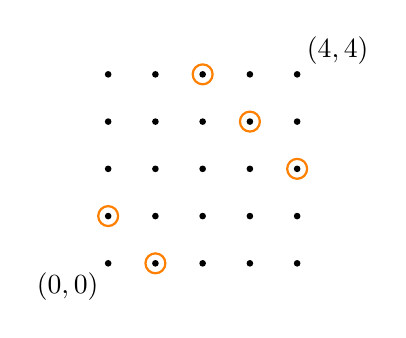
\begin{tikzpicture}[scale=0.6]
            \foreach \x in {0,...,4} \foreach \y in {0,...,4} \fill (\x,\y) circle (2pt);
            \foreach \p in {(1,0),(0,1),(4,2),(3,3),(2,4)} \draw[thick, color=orange] \p circle (6pt);
            \node[below left] at (0,0) {$(0,0)$};
            \node[above right] at (4,4) {$(4,4)$};
        \end{tikzpicture}
    \end{center}
\end{ex}

\begin{thm}[Warning's Theorem]
    Let $K = \F_q = \F_{p^f}$, $f_1,\dots,f_r \in K[x_1,\dots,x_n]$, $d = \sum \deg f_i$, and $V = V(f_1) \cap \cdots \cap V(f_r)$. If $V \neq \emptyset$, then $\# V \geq q^{n-d}$.
\end{thm}

\section{Quadratic Reciprocity}

\subsection{Preliminaries}

We want to understand the perfect squares in $\F_q^\times$.

\begin{thm}[][label=thm:squares-index-two]
    Let $q = p^f$.
    \begin{enumerate}[(1)]
        \item If $p = 2$, all elements of $\F_q$ are squares.
        \item If $p > 2$, then the squares form a subgroup of $\F_q^\times$ of index $2$.
    \end{enumerate}
\end{thm}

\begin{proof}[Proof of (1)]
    Let $K$ have characteristic $2$. Then, the map $K \to K$ given by $x \mapsto x^2$ is a homomorphism of fields. So, it must be injective, and if $K$ is finite, then the map is surjective.
\end{proof}

\begin{proof}[Proof of (2)]
    Let $\psi : \F_q^\times \to \{\pm 1\}$ be given by $\psi(a) = a^{\frac{q-1}{2}}$. Then, $\psi$ is a homomorphism of groups. Let $c = \psi(a) = a^{\frac{q-1}{2}}$. Then, $c^2 = 1$, hence $c$ is a root of $x^2 - 1 = 0$. So, $a^{\frac{q-1}{2}}$ can only be $\pm 1$.

    Now, we claim $\ker \psi = \{a \in \F_q^\times \mid \psi(a) = 1\}$ is the set of squares in $\F_q^\times$. Suppose $a \in (\F_q^\times)^2$, i.e. $a = b^2$ for some $b \in \F_q^\times$. Then, $\psi(a) = 1$. Hence, $(\F_q^\times)^2 \leq \ker \psi$. Conversely, if $a \in \ker \psi$, we need to show $a \in (\F_q^\times)^2$.

    Is $\psi$ onto? Yes: $\F_q^\times$ is cyclic, so it has a generator $g$, hence $g^{\frac{q-1}{2}} = -1$. Hence, $\F_q^\times / \ker \psi \cong \{\pm 1\}$, so $|\ker \psi| = \frac{q-1}{2}$. This means $\angles{g^2} = \ker \psi$ (a cyclic group has only one subgroup of a given order), so everything in $\ker \psi$ is a square.
\end{proof}

\begin{defn}
    Let $A, B, C$ be abelian groups, and consider homomorphisms
    $$0 \to A \arr[f] B \arr[g] C \to 0$$
    with $g(f(a)) = 0$ for all $a \in A$. This is a \textbf{sequence}. We say it's \textbf{exact on the left} if $f$ is injective, and \textbf{exact on the right} if $g$ is surjective. We say it's \textbf{exact in the middle} if $\Img f = \ker g$. We say it's an \textbf{exact sequence} if all $3$ hold.
\end{defn}

\begin{prop}
    If we have an exact sequence as above, then $B/\ker g \cong C$, so $B/\Img f \cong C$. Since $A \cong \Img f$, we have $B/A \cong C$.
\end{prop}

\begin{ex}
    The following sequences are exact:
    \begin{enumerate}
        \item $0 \to \Z \arr[\cdot 2] \Z \arr[\text{mod } 2] \Z/2\Z \to 0$
        \item $0 \to \Z \to \Q \to \Q/\Z \to 0$
        \item $1 \to \{\pm 1, \pm i\} \arr[\times] \C^\times \arr[a^4] \C^\times \to 1$. (We use $1$ instead of $0$ as a convention, since $1$ is the identity.)
        \item $1 \to (\F_q^\times)^2 \to \F_q^\times \arr[\psi] \{\pm 1\} \to 1$, where $\psi$ is the map from before.
    \end{enumerate}
\end{ex}

\begin{ex}
    Let $G$ be abelian, and consider the map $\phi_n : G \to G$ given by $\phi_n(a) = a^n$. Then, $\ker \phi_n = \{g \in G : g^n = e\}$. For example, we have the exact sequence
    $$1 \to \{\pm 1\} \to \F_q^\times \arr[\phi_2] (\F_q^\times)^2 \to 1.$$
\end{ex}

\begin{notebox*}[Principle]
    To check if $a \in \F_q^\times$ is a square, we need to check whether $\sqrt{a} = b \in \Omega$ satisfies $b^{q-1} = 1$.
\end{notebox*}

\subsection{The Legendre Symbol}

We now only consider prime fields.

\begin{defn}
    Let $a \in \Z$, and $p$ be prime. The \textbf{Legendre symbol} is
    $$\leg{a}{p} = \case{1 & \text{if } a \text{ is a square in } \F_p \\ -1 & \text{otherwise}}$$
    for $p \nmid a$, and $\leg{0}{p} = 0$.
\end{defn}

\begin{notebox*}
    $\leg{a}{p}$ depends only on the congruence class of $a$ modulo $p$.
\end{notebox*}

\begin{prop}
    If $b \in \Omega$ satisfies $b^2 = a \in \F_p^\times$, then
    $$\psi(a) = a^{\frac{p-1}{2}} = b^{p-1},$$
    which is $1$ if and only if $b \in \F_p$. So, $\leg{a}{p} = b^{p-1} \in \F_p^\times$, i.e. $\psi(a) = \leg{a}{p}$. Since $\psi(ab) = \psi(a)\psi(b)$, we have
    $$\leg{ab}{p} = \leg{a}{p} \leg{b}{p}.$$
\end{prop}

\begin{prop}
    We have
    $$\leg{a}{p} = \case{0 & a = 0 \\ 1 & a \text{ is a square} \\ -1 & a \text{ is not a square}}$$
    so $\sum_{a \in \F_p} \leg{a}{p} = 0$.
\end{prop}

Now, it helps to compute the Legendre symbol in special cases. In particular, we want to compute $\leg{-1}{p}$ and $\leg{2}{p}$.

\begin{defn}
    Let $n \in \Z$ be odd. We define two maps:
    $$\veps(n) \in \Z/2\Z, \quad \veps(n) = \frac{n-1}{2} \bmod 2 = \case{0 & n \equiv 1 \pmod 4 \\ 1 & n \equiv 3 \pmod 4}$$
    $$\omega(n) \in \Z/2\Z, \quad \omega(n) = \frac{n^2-1}{8} \bmod 2 = \case{0 & n \equiv \pm 1 \pmod 8 \\ 1 & n \equiv \pm 3 \pmod 8}$$
\end{defn}

\begin{thm}[][label=thm:legendre-special]
    Let $p$ be an odd prime. Then,
    \begin{enumerate}[(1)]
        \item $\leg{-1}{p} = (-1)^{\veps(p)}$, so $\leg{-1}{p} = 1 \iff p \equiv 1 \pmod 4$.
        \item $\leg{2}{p} = (-1)^{\omega(p)}$, so $\leg{2}{p} = 1 \iff p \equiv \pm 1 \pmod 8$.
    \end{enumerate}
\end{thm}

\begin{proof}
    \hfill
    \begin{enumerate}[(1)]
        \item If $-1 = c^2$ in $\F_p^\times$, then $c$ has order $4$. This requires $4 \mid p - 1$, i.e. $p \equiv 1 \pmod 4$, and further $p \equiv 3 \pmod 4 \implies \leg{-1}{p} = -1$. Now, suppose $p \equiv 1 \pmod 4$. Since $\F_p^\times$ is cyclic, let $\F_p^\times = \angles{g}$, so $g^{\frac{p-1}{4}} = g^k$ has order $4$. So, $-1 = (g^k)^2$, hence $\leg{-1}{p} = 1$.
        \item Let $\alpha \in \Omega$ be a primitive $8\th$ root of unity. So, $\alpha^8 = 1$, and
        \begin{enumerate}[(i)]
            \item $\alpha^4 = -1$.
            \item $\alpha^2 + \alpha^{-2} = 0$. Indeed, $(\alpha^2 + \alpha^{-2})^2 = \alpha^4 + \alpha^{-4} + 2\alpha^2\alpha^{-2} = -1 + (-1) + 2 = 0$.
            \item Let $y = \alpha + \alpha^{-1}$. Then, $y^2 = 2$. Indeed, $y^2 = (\alpha + \alpha^{-1})^2 = \alpha^2 + \alpha^{-2} + 2\alpha\alpha^{-1} = 0 + 2 = 2$.
        \end{enumerate}
        To compute $\leg{2}{p}$, we need $2^{\frac{p-1}{2}} = y^{p-1}$. Now,
        $$y^p = (\alpha + \alpha^{-1})^p = \alpha^p + \alpha^{-p}.$$
        If $p = 8k + 1$, then $y^p = \alpha^{8k+1} + \alpha^{-1-8k} = \alpha + \alpha^{-1} = y$, so $y^{p-1} = 1$, hence $y \in \F_p^\times$. Hence, $\leg{2}{p} = 1$. The case $p = 8k - 1$ is similar.

        If $p = 8k + 5$, then
        $$y^p = \alpha^{8k+5} + \alpha^{-5-8k} = \alpha^5 + \alpha^{-5} = \alpha\alpha^4 + \alpha^{-1}\alpha^{-4} = -(\alpha + \alpha^{-1}) = -y,$$
        hence $y^p = -y$, so $y^{p-1} = -1$, showing $\psi(2) = -1$, and thus $\leg{2}{p} = -1$. The case $p = 8k - 5$ is similar.
    \end{enumerate}
\end{proof}

\begin{ex}
    Let $f(x) = ax^2 + bx + c \in \F_p[x]$, with $p \nmid a$. By the quadratic formula, $f$ has roots $\iff \leg{b^2 - 4ac}{p} = 1$. In particular, $\F_p[x]/(f)$ is a field $\iff \leg{b^2-4ac}{p} = -1$.
\end{ex}

\subsection{Quadratic Reciprocity}

\begin{thm}[Quadratic Reciprocity (Carl ``G-money'' Gauss)][label=thm:qr]
    Let $p, \ell$ be odd primes, $p \neq \ell$. Then,
    $$\leg{p}{\ell} \leg{\ell}{p} = (-1)^{\veps(p)\veps(\ell)} = (-1)^{\frac{p-1}{2} \cdot \frac{\ell-1}{2}}.$$
\end{thm}

\begin{cor}
    $\leg{p}{\ell} = \leg{\ell}{p}$, unless $p \equiv \ell \equiv 3 \pmod 4$.
\end{cor}

\begin{ex}
    Let $\ell = 4003$ and $p = 5$. Computing $\leg{5}{4003}$ directly is hard, but $\leg{4003}{5}$ is easy:
    $$-1 = \leg{4003}{5} = \leg{5}{4003}.$$
\end{ex}

\begin{proof}[Proof of \Cref{thm:qr}]
    Fix $\F_p$, with $\F_p \subset \Omega$ algebraically closed. Let $\omega$ be a primitive $\ell\th$ root of unity in $\Omega$.

    \begin{lem}[][label=lem:qr0]
        $1 + \omega + \omega^2 + \cdots + \omega^{\ell - 1} = 0$.
    \end{lem}

    Also, recall that $\leg{a}{p} = b^{p-1}$ if $b^2 = a$.

    Consider the (well-defined) function $\F_\ell \to \{\pm 1\}$ given by $a \mapsto \leg{a}{\ell}$. Note that $\omega^a$ depends only on $a \bmod \ell$, so we can also consider the function $\F_\ell \to \Omega$ given by $a \mapsto \omega^a$. Let
    $$y = \sum_{a \in \F_\ell} \leg{a}{\ell} \omega^a \in \Omega.$$
    This $y$ is called a \textbf{Gauss sum}.

    \begin{lem}[][label=lem:qr1]
        $y^2 = (-1)^{\veps(\ell)} \ell$.
    \end{lem}

    \begin{lem}[][label=lem:qr2]
        $y^{p-1} = \leg{p}{\ell}$.
    \end{lem}

    We will show these lemmas imply quadratic reciprocity, and then prove them. As $y^2 = (-1)^{\veps(\ell)}\ell$, we get from the note above (with $b = y$) and \Cref{lem:qr2} that
    $$\leg{(-1)^{\veps(\ell)}\ell}{p} = y^{p-1} = \leg{p}{\ell}.$$
    As the Legendre symbol is multiplicative,
    $$\leg{(-1)^{\veps(\ell)}\ell}{p} = \leg{-1}{p}^{\veps(\ell)} \leg{\ell}{p} = \paren{(-1)^{\veps(p)}}^{\veps(\ell)} \leg{\ell}{p}.$$
    So, $\leg{p}{\ell} = (-1)^{\veps(p)\veps(\ell)} \leg{\ell}{p}$, hence
    $$\leg{p}{\ell}\leg{\ell}{p} = (-1)^{\veps(p)\veps(\ell)},$$
    as desired.
\end{proof}

\begin{proof}[Proof of \Cref{lem:qr0}]
    As $\omega$ is a primitive $\ell\th$ root of $1$, $\omega$ is a root of
    $$\frac{x^\ell - 1}{x - 1} = 1 + x + \cdots + x^{\ell - 1},$$
    so $1 + \omega + \cdots + \omega^{\ell - 1} = 0$.
\end{proof}

\textit{(Rama really wants us to understand this proof.)}

\begin{proof}[Proof of \Cref{lem:qr2}]
    Let $y = \sum_{a \in \F_\ell} \leg{a}{\ell} \omega^a$. As $\Omega$ has characteristic $p$,
    $$y^p = \paren{\sum \leg{a}{\ell} \omega^a}^p = \sum_{a \in \F_\ell} \leg{a}{\ell}^p \omega^{ap} = \sum \leg{a}{\ell} \omega^{ap}.$$
    Let $c = ap \in \F_\ell$, so that $a = cp^{-1} \in \F_\ell$. So, we have
    $$\sum_{c \in \F_\ell} \leg{cp^{-1}}{\ell} \omega^c = \sum \leg{c}{\ell}\leg{p^{-1}}{\ell} \omega^c = \leg{p^{-1}}{\ell} \sum_{c \in \F_\ell} \leg{c}{\ell} \omega^c.$$
    Note that $\leg{p}{\ell}\leg{p^{-1}}{\ell} = 1$, so $\leg{p}{\ell} = \leg{p^{-1}}{\ell}$. Hence, this equals
    $$\leg{p}{\ell} \sum_{c \in \F_\ell} \leg{c}{\ell} \omega^c = \leg{p}{\ell} y.$$
    So, $y^p = \leg{p}{\ell} y$, hence $y^{p-1} = \leg{p}{\ell}$.
\end{proof}

\begin{proof}[Proof of \Cref{lem:qr1}]
    Note the following:
    \begin{itemize}
        \item The map $\F_\ell^\times \to \F_\ell^\times$ given by $t \mapsto t^{-1}$ is bijective.
        \item For $u \in \F_\ell^\times$, the maps $t \mapsto ut$ and $t \mapsto -ut$ are bijections.
        \item The map $\F_\ell \to \F_\ell$ given by $t \mapsto t + 1$ is a bijection, and $\F_\ell^\times$ is mapped to $\F_\ell \setminus \{1\}$.
    \end{itemize}
    Now, we want to show $y^2 = (-1)^{\veps(\ell)}\ell$. By definition,
    \begin{align*}
        y^2 = y \cdot y &= \paren{\sum_{x \in \F_\ell} \leg{x}{\ell} \omega^x}\paren{\sum_{z \in \F_\ell} \leg{z}{\ell} \omega^z} \\
        &= \sum_{x,z \in \F_\ell} \leg{x}{\ell}\leg{z}{\ell} \omega^{x+z} = \sum \leg{xz}{\ell} \omega^{x+z}.
    \end{align*}
    For $u \in \F_\ell$, we want the coefficient of $\omega^u$, so $x + z = u$, i.e. $z = u - x$. We now have
    $$y^2 = \sum_{u \in \F_\ell} B_u \omega^u, \qquad \text{where } B_u = \sum_{t \in \F_\ell} \leg{t(u-t)}{\ell}.$$
    Now,
    \begin{align*}
        B_u &= \sum_{t \in \F_\ell} \leg{t(u-t)}{\ell} = \sum_{t \in \F_\ell^\times} \leg{t(u-t)}{\ell} = \sum_{t \in \F_\ell^\times} \leg{-t^2(1-ut^{-1})}{\ell} \\
        &= \sum \leg{-1}{\ell}\leg{t^2}{\ell}\leg{1-ut^{-1}}{\ell} = \sum (-1)^{\veps(\ell)} \leg{1-ut^{-1}}{\ell} = (-1)^{\veps(\ell)} \sum_{t \in \F_\ell^\times} \leg{1-ut^{-1}}{\ell}.
    \end{align*}
    So, let $B_u = (-1)^{\veps(\ell)} C_u$, where $C_u = \sum_{t \in \F_\ell^\times} \leg{1-ut^{-1}}{\ell}$. For $u = 0$,
    $$C_0 = \sum_{t \in \F_\ell^\times} \leg{1}{\ell} = \ell - 1.$$
    Now, if $u \neq 0$, then $t \mapsto t^{-1} \mapsto -ut^{-1} \mapsto 1 - ut^{-1}$ is a bijection $\F_\ell^\times \to \F_\ell \setminus \{1\}$. So,
    $$C_u = \sum_{t \in \F_\ell^\times} \leg{1-ut^{-1}}{\ell} = \sum_{s \in \F_\ell \setminus \{1\}} \leg{s}{\ell} = -1 + \sum_{s \in \F_\ell} \leg{s}{\ell} = -1.$$
    Hence, using \Cref{lem:qr0},
    \begin{align*}
        y^2 = \sum_{u \in \F_\ell} B_u \omega^u = (-1)^{\veps(\ell)} \sum C_u \omega^u &= (-1)^{\veps(\ell)} \paren{\ell - 1 + \paren{\sum_{u \in \F_\ell^\times} \omega^u}(-1)} \\
        &= (-1)^{\veps(\ell)}(\ell - 1 + 1) = (-1)^{\veps(\ell)}\ell.
    \end{align*}
\end{proof}


\newpage
\notechapter{\texorpdfstring{$p$-Adic Fields}{p-Adic Fields}}
% !TEX root = ../math407-notes.tex

\section{\texorpdfstring{The Ring $\Z_p$ and the Field $\Q_p$}{The Ring Zp and the Field Qp}}

\begin{defn}
    An \textbf{inverse system} of sets/groups/rings/(category) is
    \begin{enumerate}
        \item[(i)] A sequence $A_n$ of sets/groups/rings and
        \item[(ii)] A sequence of morphisms
        $f_n:A_n\to {A_{n-1}}$
    \end{enumerate}
    $$\cdots \to A_3 \overset{f_3}{\to}A_2\overset{f_2}{\to}A_1$$
\end{defn}

\begin{defn}
    The \textbf{inverse limit} of the system $(A_n,f_n)_{\geq 1}$ is $A =\underset{\leftarrow}{\lim}A_n$ defined as $A=\{ (\dots,a_2,a_1) \mid a_n\in A_n,f_n(a_n)=a_{n-1} \:\: \forall n \geq 2 \}$. Note then that $A \subset \prod_{n\geq1}A_n$
\end{defn}

\begin{ex}[Main example]
    Let $p$ be a prime number, $A_n= \Z/p^n\Z$, $\phi_n:A_n \to A_{n-1}$, defined by $\bar a \mapsto a \pmod {p^{n-1}}$. Note that $\phi_n$ are all surjective. We then define $\Z_p = \underset{\leftarrow}{\lim}A_n$, called the \textbf{p-adic integers}, a ring. In particular, if $\vec{a}=(\dots,a_2,a_1)$ and $\vec b=(\dots,b_2,b_1)$, then $\vec a + \vec b = (\dots,a_2+b_2,a_1+b_1)$ and $\vec a \cdot \vec b=(\dots,a_2b_2,a_1b_1)$, and one can verify these remain in the p-adic integers
\end{ex}

\begin{ex}
    In $\Z_p$, we have multiplicative identity $\vec 1 = (\dots,1,1,1)$ and the additive identity $\vec 0 =(\dots,0,0)$. For any $m\in \Z$, we can look at $\vec m=(\dots,m,m,m)$. Thus, we have a map $\Z \to \Z_p$ by $m \mapsto \vec m$, which is also a homomorphism. Suppose $m \in \Z$ satisfies $\vec m = \vec 0$. Then, we must have $m=0$, hence the kernel of the map is trivial. (We can sort of say $\Z_p$ is a characteristic $0$ ring, which will be more important later)
\end{ex}

\begin{ex}[What else is in $\Z_p$]
    $1/2 \not \in \Z$, but we do have $1/2 \in \Z_7$. We also have $\sqrt 2 \in \Z_7,2^{1/5}\in \Z_7$, but $2^{1/3}\not \in \Z_7$
\end{ex}

\begin{defn}
    We have a homomorphism $\veps_n :\Z_p \to A_n=\Z /p^n\Z$ by $\veps_n(\vec a)= a_n$
\end{defn}

\begin{thm}[][label=thm:zp-exact]
    There exists an exact sequence $0 \to \Z_p \overset{\cdot p^n}{\to} \Z_p \overset{\veps_n}{\to}A_n\to0$, so $\veps_n$ is surjective, and we'll also show multiplication by $p^n$ is injective. This also says $\Z_p/p^n\Z_p \cong \Z / p^n\Z$.
\end{thm}

\begin{proof}
    Consider the map $\Z_p \to \Z_p$ by $\vec a \mapsto p\vec a$. Observe that for $c \in \Z/p^n\Z$, we have that $pc=0 \implies p^{n-1} \mid c$. Now, suppose $\vec a \in \Z_p$ satisfies $p\vec a = \vec 0$, so $pa_1=0 \in A_1$, $pa_2=0\in A_2$, etc. This means that for all $n$, $pa_n = 0 \in A_n=\Z/p^n\Z$, thus $a_n=p^{n-1}b_n$ for some $b_n \in A_n$. By $\vec a \in \Z_p$, we know $\phi(a_n)=a_{n-1},\phi(n+1)=a_n$, etc. Furthermore,
    $$a_{n}=\phi(a_{n+1})=\phi(p^{n}b_{n+1})=p^{n}\phi(b_{n+1})=0\in A_{n}.$$
    Thus, $\vec a =0$, so multiplication by $p$ is injective, and it follows that multiplication by $p^n$ is injective.

    Now, for any $\bar c \in \Z/p^n\Z$, we have that $\veps _n(\dots,c,c,c)=\bar c$, hence $\veps _n$ is surjective.

    Finally, we'll show $\ker \veps _n = p^n \Z _p$. $p^n \Z_p \subset \ker \veps _n$ is clear. Let $\vec a \in \ker \veps _n$. We want to show $\vec a = p^n\vec b$ for $\vec b \in \Z^p$. As $\vec a \in \ker \veps_n$, we know $a_n=0\implies a_{n-1}=0=a_{n-2}+\cdots=a_1$. Now, consider $A_{n+1} \overset{\phi _{n+1}}{\to} A_n$ by $a_{n+1}\mapsto a_n=0$, hence $a_{n+1} \in \ker \phi_{n+1}$, so $a_{n+1}=p^nb_{n+1}$. A similar argument can be made for $a_{n+2}$ with composing maps, and inductively we have $a_{n+j}=p^nb_{n+j}$. So, it's left to us to check $(\dots,b_{n+2},b_{n+1},b_n,\dots,b_1)\in \Z_p$.
\end{proof}

\begin{ex}[Another inverse system]
    Let $K$ be a field, $R=K[x]$, $B_n=K[x]/(x^n)=R/(x^n)$. What is $B= \underset{\leftarrow}{\lim}B_n$?
\end{ex}

\begin{notebox*}[Question]
    What is $\Z_7^\times$?
\end{notebox*}

For $\vec a = (a_n ) \in \prod A_n$ to be a unit, we certainly need $a_n$ is a unit in $A_n$.

\begin{thm}[Structure of Units][label=thm:zp-units]
    Let $a \in \Z_p$, $a \neq 0$. Then
    \begin{enumerate}
        \item $\vec a$ unit in $\Z_p \iff a_1 \in \F_p^\times = (\Z/p\Z)^\times$
        \item Let $U = \Z_p^\times$ in $\Z_p$.  Then, any $a \in \Z_p$ non-zero can be written as $p^n\vec b$ for $n \geq 0$ and $\vec b\in U$ uniquely.
    \end{enumerate}
\end{thm}

\begin{proof}
    \begin{enumerate}
        \item $( \implies)$ obvious.
    \end{enumerate}

    Now, let $a \in \Z_p$ with $a_1 \in \F_p^\times$. We want to show $a_n \in A_n^\times$ for all $n \geq 1$. Let $a_1^{-1}=b_1$, and as $A_2 \to A_1$ is surjective, for $a_2$ mapping to $a_1$, there exists some $b_2 \in A_2$ which is mapped to $A_1$. Then $\phi_2(a_2b_2)=1=\phi_2(1)$, so $a_2b_2-1 \in \ker \phi_2$. Hence, $a_2b_2 = 1-pz$ for some $z \in A_2$. Now, $a_2b_2(1+pz)=(1-pz)(1+pz)=1-p^2z=1$. In general, for $a_n \mapsto a_1$, there exists some $b_n \mapsto b_1$, and once again $a_nb_n-1 \in \ker(\Z/p^n\Z \to \Z/p\Z)$. Thus, $a_nb_n=1-pz$. Recall $(1-t)(1+t+\cdots +t^{n-1})=(1-t^n)$. Hence, $a_nb_n(1+pz+p^2z^2+\cdots +p^nz^n) = 1-p^nz^n=1$.
\end{proof}

\begin{cor}
    $m \in \Z_p^\times$ if $p \nmid m$.
\end{cor}

\begin{proof}[Proof of (2) of \Cref{thm:zp-units}]
    Suppose $\vec a \in \Z_p$ is nonzero. Then, $\veps_m(\vec a) \neq 0$ for some $m$. Let $n$ be the largest integer such that $\veps _n(\vec a)=0$, recalling that $\veps_{n-k}(\vec a)=0$ for all $k \geq 0$. In particular, $\vec a \in \ker \veps _n \implies \vec a = p^n\vec b$ for some $\vec b \in \Z_p$ by \Cref{thm:zp-exact}. Now, \textbf{show $b_1 \neq 0$}. Thus, $\vec b$ is a unit in $\Z_p$, proving (2).
\end{proof}

\begin{defn}
    If $\vec a \in \Z_p$ is nonzero, then we know $\vec a = p^n\vec b$ for $\vec b$ a unit and $n \geq 0$. So, let the \textbf{$p$-adic valuation} of $\vec a$ by $\nu_p(\vec a)=n$. Note $\nu_p(\vec a) = 0 \iff a$ is a unit in $\Z_p$. We will also declare $\nu_p(0) = \infty$.
\end{defn}

\begin{rmk}
    $\nu_p(\vec a \vec b)=\nu_p(\vec a)+\nu _p(\vec b)$, and $\nu_p(a+b) \geq \min \{\nu _p(a),\nu _p(b)\}$. We call this \textbf{non-Archimedean equality}.
\end{rmk}

\begin{cor}
    $\Z_p$ is an integral domain.
\end{cor}

\begin{proof}
    If $a,b$ are non-zero, then they have finite $p$-adic valuation, so the $p$-valuation of their product is also finite.
\end{proof}

\begin{defn}[$\Q_p$]
    Let $\Q_p$ be the field of fractions of $\Z_p$, i.e. the smallest field containing $\Z_p$.
\end{defn}

\begin{rmk}
    For any $a \neq 0$, let $a=p^nb$, where $b$ is a unit. Then, the inverse of $a$ in $\Q_p$ is $p^{-n}b^{-1}$. It's worth noting that $b^{-1} \in \Z_p$, so the only thing we have to 'add' is $p^{-n}$. Thus, $\Q_p = \Z_p[1/p]$.
\end{rmk}

Let's make $\Z_p$ more concrete. Recall $\Z_p = \underset{\leftarrow}{\lim}\Z/p^n\Z$.

Let $\vec a = (a_n)$, and for the usual map $\Z/{p^{n+1}}\Z \to \Z/p^n\Z$, consider $a_{n+1}\mapsto a_n$, where $a_{n+1}\in \{0,\dots,p^{n+1}-1\}$ and $a_n \in \{0,\dots,p^n-1\}$. So, we can see that $a_{n+1}=a_n+p^nb_n$, with $0 \leq b_n \leq p-1$. This is like $31$ mod $100$ and $31,131,\dots,931$ mod $1000$. Now, consider the sequence $b_0=a_1,b_1=\frac{a_2-a_1}{p},b_2=\frac{a_3-a_2}{p},\dots,b_n=\frac{a_{n+1}-a_n}{p^n},\dots$. By definition,
$$a_n=b_0+b_1p+\cdots+b_{n-1}p^{n-1}$$.

\begin{defn}[$p$-adic Expansion]
    The sequence $(b_0,b_1,\dots)$ described above is called the \textbf{$p$-adic expansion of $\vec a$}
\end{defn}

\begin{thm}
    There is a bijection between $\Z_p \longleftrightarrow $ sequences $(b_n)$, with $b_i \in \{0,\dots,p-1\}$
\end{thm}

\begin{proof}
    For $\vec a \in \Z_p$, we showed above how to obtain $(b_n)$ by $b_n=\frac{a_{n+1}-a_n}{p^n}$ Conversely, let $(b_n)$ be such a sequence. We can take the formula with which we constructed the $b_n$'s earlier to try $a_1=b_0,a_2=b_0+pb_1,a_3=b_0+pb_1+p^2b_2$, and generally $a_n=b_0+\cdots +b_{n-1}p^{n-1}$. Indeed, for the map $\Z/p^{n+1}\Z \to \Z/p^n\Z$, observe
    $$b_0+\cdots+b_{n-1}p^{n-1}+b_np^n \mapsto b_0+\cdots +b_{n-1}p^{n-1},$$
    so we indeed have a $p$-adic integer. Check that this relation is bijective.
\end{proof}

\begin{ex}
    $1+1\cdot 3+1\cdot 3^2+\cdots$ is like the power series $\frac 1{1-x}$, so this  is the $p$-adic expansion of $\frac{1}{-2}$.

    If $\vec a=b_0+b_1p+b_2p^2+\cdots \longleftrightarrow (b_0,b_1,\dots)$, then $p\vec a \longleftrightarrow (0,b_0,b_1,\dots,)$
\end{ex}

Let's revisit the sequence $0 \to \Z_p \overset{p^n}{\to}\Z_p \overset{\veps_n}{\to}\Z/p^n\Z\to 0$. Let's show $\ker \veps _n = p^n\Z_p$. $\vec a \in \ker \veps _n \iff a_n=0 \implies a_{n-1}=\cdots =a_1=0$, so the $p$-adic expansion of $\vec a$ is $(0,\overset{n}{\cdots},0,a_{n+1},\dots)$, which we see is in $p^n\Z_p$, like in the example above. This is the analog of saying "an integer with three zeroes at the end must be divisible by $1000$".

\section{\texorpdfstring{The $p$-Adic Absolute Value}{The p-Adic Absolute Value}}
\begin{defn}[The $p$-adic Absolute Value]
    The \textbf{$p$-adic absolute value} of $\vec a$ is $|\vec a|_p=\frac{1}{p^{\nu_p(a)}}$. In particular, the higher the $p$-valuation of a number is, the 'smaller' it is. Note $|0|_p=\frac{1}{p^\infty}=0$
\end{defn}

\begin{rmk}
    Before, we said $1+1\cdot 3 +1\cdot 3^2+\cdots$, is $\frac{1}{1-3}$ because it's a geometric series. We now see this is ok, because $|p|_p=\frac{1}{p}<1$.
\end{rmk}

\begin{ex}
    Let $a \in \Z_5$, $a=\sum_{i=0}^\infty b_ip^i$. We can practice finding expansions

    $-1=5-1-5=4+5(-1)=4+4\cdot 5-25=4+4\cdot5 +25(-1)=\cdots$

    $-1=(\dots,4,4,4)$
\end{ex}

\begin{prop}[Properties of the $p$-adic Absolute Value]
    $|a|_p\geq0$, and $|a|_p=0\iff a$ is a unit. $|ab|_p=|a|_p|b|_p$, and $|a+b|_p \leq \max\{|a|_p,|b|_p\}$. This is the \textbf{ultrametric inequality}
\end{prop}

\begin{defn}[Distance on $\Z_p$]
    For $a,b \in \Z_p$, we define $d(a,b)=|a-b|_p$. Observe that $d(a,a)=0$, $d(a,b)=d(b,a)$, and $d(a,b)+d(b,c) \geq d(a,c)$. In fact, $|a-c|_p \leq \max\{|a-b|_p,|b-c|_p\}$, which is an even stronger version of the triangle inequality, called a \textbf{non-Archimedean inequality}.
\end{defn}

Note that $p$-adic valuation can be extended to $\Q_p$, and we have that $|a|_p \leq 1 \iff a \in \Z_p$.

\begin{ex}
    $|a|_p = 1/p \iff a \in p\Z_p\setminus p^2\Z_p$

    $|a|_p=1/p^2 \iff a \in p^2\Z_p \setminus p^3\Z_p$

    In general, we can think of $\Z_p$ as the closed unit disk with radius less than $1$, and it's a union of circles like that. We can also see
    $$\Q_p \setminus \{ 0\} =\sqcup_{n\in \Z}p^n\Z_p^\times$$
\end{ex}

\begin{prop}
    Any triangle in $\Q_p$ is isosceles.
\end{prop}

\begin{proof}
    With one vertex of the triangle at $0$, let the edges be $x,y,y-x$, then $|x-y|_p \leq \max\{|x|_p,|y|_p\}$. Suppose $|x|_p <|y|_p$. Then, $|x-y|_p\leq |y|_p$. On the other hand, $|y|_p=|x-(x-y)|_p\leq \max\{|x|_p,|x-y|_p\}$. Since we assumed $|y|_p \not \leq |x|_p$, we must have $|y|_p \leq |x-y|_p$. Thus, $|y|_p=|x-y|_p$, proving the triangle is isosceles.
\end{proof}

\begin{prop}
    We may define $B_r(a)$ to be the disk of radius $r$ centered at $a\in \Z_p$, $\{x \in \Q_p : |x-a|_p < r\}$. Then, if $b \in B_r(a)$, we have that $B_r(a)=B_r(b)$.
\end{prop}

\begin{proof}
    Exercise.
\end{proof}

Let $K$ be a field, and let $A_n=K[t]/(t^n)$. Then, there is a ring homomorphism $\phi_n:A_n \to A_{n-1}$ by $\phi(a_0+a_1t+\cdots+a_nt^n)=\phi(a_0+a_1t+\cdots+a_{n-1}t^{n-1})$. We then get an inverse limit $\underset{\leftarrow}{\lim}K[t]/(t^n)$, which is the power series ring $K[[t]]$.

\begin{defn}
    Let $K$ be a field. An \textbf{absolute value} ok $K$ is a map $|\cdot|:K \to \R$ such that
    \begin{enumerate}
        \item $|x|>0$ unless $x=0$. $|0|=0$.
        \item $|xy|=|x||y|$
        \item $|x+y| \leq |x| + |y|$ (Triangle Inequality)
    \end{enumerate}
    We say that an absolute value is \textbf{non-Archimedean} if $|x+y| \leq \max\{|x|,|y|\}$.
\end{defn}

\begin{ex}
    We have the usual absolute value over $\Q$: $|a|_\infty =\sqrt{a^2}$. We have also shown that $|\cdot |_p:\Q \to \R$ is an absolute value for any prime $p$.
\end{ex}

\begin{ex}
    Let $c \in K$ be a root of unity. As $c^n=1$, we also have $|c|^n=1$, so $|c|=\pm1 \implies |c|=1$.
\end{ex}

\begin{defn}
    For $K$ any field, we have the \textbf{trivial absolute value} $|a|=1,|0|=0$.
\end{defn}

\begin{prop}
    When $K$ is a finite field, the trivial absolute value is the only absolute value.
\end{prop}

\begin{defn}
    Let $|\cdot|_1,|\cdot|_2$ be absolute values on $K$. We say they are \textbf{equivalent} if $|\cdot |_1=|\cdot |_2^c$ for some $c \in \R_{>1}$
\end{defn}

\begin{ex}
    Instead of $|a|_p=\frac{1}{p^{\nu_p(a)}}$, we can use $|a|_p=\frac{1}{e^{\nu_p(a)}}$, which is equivalent.
\end{ex}

\begin{prop}
    $|\cdot |_1$ and $|\cdot |_2$ are equivalent if for any $a \in K$, $|a|_1 < 1 \iff |a|_2 < 1$. Furthermore, a sequence $\{a_n\}_{n \geq 1}$ is Cauchy with respect to $|\cdot |_1$ iff it's Cauchy with respect to $|\cdot |_2$.
\end{prop}

\begin{defn}
    A sequence $\{a_n\}_{n\geq 1}$ on $K$ is \textbf{Cauchy} with respect to $|\cdot |$ if for any $\varepsilon>0$, there exists $N \in \N$ such that $n,m\geq N \implies |a_n-a_m| < \varepsilon$.

    Furthermore, we say $K$ is \textbf{complete} with respect to $|\cdot |$ if every Cauchy sequence has a limit in $K$.
\end{defn}

For example, $\R$ is complete with respect to the usual absolute value, but $\Q$ is not complete with both the usual absolute value and $|\cdot |_p$.

\begin{thm}
    $\Q_p$ is the completion of $\Q$ with respect to $|\cdot |_p$.
\end{thm}

\begin{thm}[Ostrowski's Theorem]
    Any non-trivial absolute value on $\Q$ is equivalent to $|\cdot |_\infty$ or $|\cdot |_p$ for some prime $p$. Furthermore, if $p \neq q$ are distinct primes, than $|\cdot |_p$ is not equivalent to $|\cdot |_q$.
\end{thm}

\begin{thm}[Product Formula]
    Let $a \in \Q$ non-zero. Then,
    $$\prod_{p \leq \infty}|a|_p=1$$
    This product is well defined because only finitely many $|a|_p \neq 1$.
\end{thm}

\begin{ex}
    Let $a=10$. Then, $|10|_2=\frac 12,|10|_3=1,|10|_5=\frac 15,|10|_7=1,|10|_n=1$ for $n \geq 11$, and $|10|_\infty =10$.
\end{ex}

\begin{proof}
    If $a$ is some prime $p$, then $|p|_p=\frac 1p,|p|_q=1,|p|_\infty=p$, so the claim holds for primes.

    Now, define $\phi:(\Q^\times,\times) \to (\R^\times,\times)$ by $\phi(a)=\prod_{p \leq \infty}|a|_p$. Then $\phi$ is a homomorphism, as $\phi(ab)=\phi(a)\phi(b)$. One can confirm that $\phi(-1)=1$, and we showed $\phi(p)=1$. Furthermore, $\phi(p)=1 \implies \phi(p^n)=1$ for any $n \in \Z$. Now, for any $a \in \Q^\times$, we have $a = \pm p_1^{e_1}\cdots p_n^{e_n}$, and the claim for $\phi(a)$ follows.
\end{proof}

\begin{rmk}
    Suppose $\{a_n\}$ is a sequence in $\R$ such that for any $\varepsilon>0$, there exists $N >1$ with $|a_{n+1}-a_n|<\veps$ for any $n> N$. This is a weaker condition than being Cauchy in $\R$. However, in $\Q_p$, this condition is equivalent to being Cauchy, as $|\cdot |_p$ is non-Archimedean.

    Thus, for a sequence $\{a_n\}$ in $\Q_p$ to converge, all that is needed is that for any $\veps >0$, there exists $N \in \N$, $n \geq N \implies |a_{n+1}-a_n|_p<\veps$. Consequently, any series $\sum_{n=1}^\infty x_n$ converges in $\Q_p$ so long as $\{x_n\}$ converges.

    This is another reason why we can say $b_0+b_1p+b_2p^2+\cdots$ is well defined in $\Q_p$.
\end{rmk}

\begin{ex}
    The sequence $1,1/2,1/3,\dots$ converges in $\R$, but diverges in $\Q_p$.
\end{ex}

\begin{prop}
    The sequence $\{u_n\}_{n \geq 1}$ converges in $\Q_p$ if and only if $\lim_{n \to \infty}|u_n-u_{n-1}|_p=0$. Similarly, $\sum_{n=1}^\infty b_n$ converges if and only if $\lim_{n \to \infty}|b_n|_p=0$
\end{prop}

\section{The Exponential Function}

\begin{notebox*}[Recall]
    $$\exp(x)=\sum_{n=0}^\infty \frac{x^n}{n!}$$
\end{notebox*}
We are curious about the convergence of this series when $x \in \Z_p$.

\begin{notebox*}[Question]
    What is $|x^n/n!|_p$?
\end{notebox*}

Let $n=b_0+b_1p+b_2p^2+\cdots +b_rp^r$, where $0 \leq b_i \le p-1$. Then, $\nu_p(n!)=\lfloor n/p\rfloor + \lfloor n /p^2\rfloor + \cdots + \floor{n/p^r}$. Observe that
$$\floor{n/p}=b_1+b_2p+b_3p^2+\cdots+b_rp^{r-1}$$
$$\floor{n/p^2}=b_2+b_3p+b_4p^2+\cdots +b_rp^{r-2}$$
$$\floor{n/p^r}=b_r$$
Thus,
\begin{prop}
    $$\nu_p(n!)=b_0\frac{p^0-1}{p-1}+b_1\frac{p^1-1}{p-1}+b_2\frac{p^2-1}{p-1}+\cdots +b_r\frac{p^r-1}{p-1}=\frac{n-\sum b_i}{p-1}$$
\end{prop}
Now,
$$\nu_p(x^n/n!)=\nu_p(x^n)-\nu_p(n!)=n(\nu_p(x) - \frac{1}{p-1})+\frac{\sum b_i}{p-1}$$
From this, we see $\nu_p(x^n/n!) \to \infty$ if $\nu_p(x) \geq \frac{1}{p-1}$.
\begin{prop}
    If $|x|_p < \frac{1}{p^{1/(p-1)}}$, then, $\exp(x)$ converges.
\end{prop}

\section{Roots of Polynomials}

Let $f(x) = x^2+1$, and we want to find roots in $\Z_5$. Note that if $f$ has a root like $f(a)=0$ is $\Z_p$, then $f$ has a root in $\Z/p^n\Z$ for every $n$.

$f(x)$ has a root in $A_1=\Z/5\Z$, for example $x=2$. Suppose $a_n$ is a root of $f(x)$ in $A_n=\Z/5^n\Z$. That is, $a_n^2+1 \equiv 0 \pmod {5^n}$. We want to find a root $a_{n+1}$ in $A_{n+1}$. Note that we need $a_{n+1}=a_n+p^{n}b_n$ for $0 \leq b_n \leq p-1$. Observe
$$a_{n+1}^2+1=(a_n+p^nb_n)^2+1=a_n^2+2\cdot 5^na_nb_n+5^{2n}b_n^2+1 \equiv a_n^2 + 2\cdot 5^na_nb_n+1 \pmod {5^{n+1}}$$
So, $2\cdot 5^na_nb_n \equiv -(a_n^2+1) \pmod{5^{n+1}}$, but $a_n^2+1$ is $0$ in $A_n$, so $a_n^2+1=5^nd_n$, thus
$$2\cdot 5^n a_nb_n\equiv 5^nd_n \pmod{5^{n+1}} \iff 2 a_nb_n \equiv d_n \pmod 5.$$
Modulo $5$, we assumed $a_n \equiv 2 \pmod 5$, so $4b_n \equiv d_n\pmod 5$. As $4$ is a unit modulo $5$, we can indeed properly solve for a $b_n$.

In this particular case there is a nice formula for the $5$-adic root of $x^2+1$: Newton's binomial formula says $(1-x)^{1/2}=\sum_{n=0}^\infty (-1)^n\binom{1/2}{n}x^n$. We are looking for $\sqrt{-1}$, and observe
$$\sqrt{-1}=\frac{1}{2}\sqrt{1-5}=\sum_{n=0}^\infty (-1)^n\binom{1/2}{n}5^n,$$
which converges in $\Z_5$.

\begin{notebox*}[Question]
    What is the algebraic closure of $\Q_p$? To close $\R$, we only need to add $i$. What are the irreducible polynomials in $\Q_p$? How do we check if a polynomial has roots.
\end{notebox*}

\begin{notebox*}[Observe]
    Let $f(x) \in \Q_p[x]$. We can multiply (or divide) $f$ by an appropriate power of $p$ so that $f$ becomes a polynomial in $\Z_p[x]$, with not all coefficients divisible by $p$.
\end{notebox*}

\begin{rmk}
    Let $f(x) \in \Z_p[x]$ with $f(a)=0$. Then, $f(\bar a) \equiv 0 \pmod {p^n}$ for all $n$. This follows from $\veps _n:\Z_p \to \Z/p^n\Z$ being a ring homomorphism.
\end{rmk}

\begin{notebox*}[Question]
    If $f$ has a root in $\Z/p^n\Z$ for all $n$, does $f$ have a root in $\Z_p$? More generally, let $f(x_1,\dots,x_n) \in \Z_p[x_1,\dots,x_n]$. Then, we ask if $V_n(f)$ nonempty implies $V(f)$ is nonempty.
\end{notebox*}

\begin{defn}[General Inverse Limits]
    Let $D_1,D_2,\dots$ be sets, with \textbf{transition maps} $D_{n+1}\to D_n$. Then, let $D$ be the \textbf{inverse limit} of $D_n$, i.e. $(d_n) \in D$ if $d_{n+1} \mapsto d_n$ for all $n$.
\end{defn}

\begin{lem}[][label=lem:nonemptylem]
    If $D_n$'s are all finite and nonempty, then $D$ is nonempty.
\end{lem}

\begin{proof}
    The conclusion is clear if all transition maps are surjective. Our idea to prove it in general is to reduce to this case.

    Fix $n \geq 1$. Let $D_{n,1}= \Img (D_{n+1} \to D_n),D_{n,2}=\Img(D_{n+2} \to D_{n+1} \to D_n)$, and generally
    $$D_{n,k}= \Img(D_{n+k} \to D_n).$$
    Observe that $D_n \supset D_{n,1} \supset D_{n,2} \supset \cdots$. By our assumption, $D_{n,k}$ are all finite and nonempty. So, there exists a $K>>0$ such that $D_{n,k}=D_{n,k+1}$ for all $k \geq K$. Call $E_n$ the set which they stabilize to. In the homework, we will prove $E_{n+1}$ surjects onto $E_n$. It follows that $\lim E_n \hookrightarrow  \lim D_n$, and by surjectivity $\lim E_n$ is nonempty.
\end{proof}
\[\begin{tikzcd}
	{E_{n+1}} && {E_n} \\
	\\
	{D_{n+1}} && {D_n}
	\arrow[two heads, from=1-1, to=1-3]
	\arrow[tail reversed, from=1-1, to=3-1]
	\arrow[tail reversed, from=1-3, to=3-3]
	\arrow[from=3-1, to=3-3]
\end{tikzcd}\]

$V_{n+1}(f) \to V_n(f)$ is a transition map, so if they're all nonempty, it follows from \Cref{lem:nonemptylem} that $V(f)$ is nonempty.

\begin{thm}
    Let $f \in \Z_p[x_1,\dots,x_n]$, $V(f)$ be the solution set of $f$, and $V_n(f)$ be the solution set of $f$ in $\Z/p^n\Z$. Then, $V(f) \neq \emptyset \iff V_n(f) \neq \emptyset$ for all $n \in \Z_+$.
\end{thm}

\begin{prop}[Special Case of Hensel's Lemma]
    Let $f(x) \in \Z_p[x]$. Let $a_0\in \F_p$ be a simple root of $f$ mod $p$. That is, $f'(a_0) \not \equiv 0 \pmod p$. Then, there exists a unique root $a$ of $f(x)$ with $a \equiv a_0 \pmod p$.
\end{prop}

\begin{proof}
    We will construct a Cauchy sequence $\{a_n\}$ in $\Z_p$, and show that $a = \lim_{n \to \infty}a_n$ satisfies $f(a)=0$. Suppose $a_n \in \Z_p$ with the property $f(a_n) \equiv 0 \pmod {p^{n+1}}$ and $a_n \equiv a_0 \pmod p$. Now, let $a_{n+1}=a_n + hp^{n+1}$ for $h \in \Z_p$, and we want to have $f(a_{n+1}) \equiv 0 \pmod {p^{n+2}}$. Well, $f(a_n+hp^{n+1})=f(a_n) + hp^{n+1}f'(a_n)+(0)$. Let $h = -f(a_n)/p^{n+1} \cdot f'(a_n)^{-1}=-c_n\cdot f'(a_n)^{-1}$, and we know $f'(a_n)$ is a unit in $\Z_p$ by assumption. Moreover, $a_{n+1}-a_n=h\cdot p^{n+1}$, so $|a_{n+1}-a_n|_p \leq \frac{1}{p^{n+1}}$, hence $a_n$ is a Cauchy sequence, and the claim follows.
\end{proof}

\begin{ex}
    Let $f(x) = x^p-x \in \Z_p[x]$. In $\F_p[x]$, we have $f(x) = x(x-1)\cdots (x-p+1)$, and these are all simple roots. It follows that $x^p-x$ has $p$ distinct roots in $\Z_p$. Moreover, $x^p-x=x(x^{p-1}-1)$, so $\Q_p$ contains the $p-1$'th roots of unity.
\end{ex}

\begin{ex}
    Let $f:\R\to \R$ be real analytic (or $f: \C \to \C$ holomorphic). Suppose $f(5) =0$. If we're looking for the multiplicity of $5$ as a root of $f$, we can look at $f'(5),f''(5),$ etc. until $f^{(n)}(5)\neq 0$. If $n$ is minimal, we can say $\nu_5(f)=n$. Moreover, $\nu_5(fg)=\nu_5(f) + \nu_5(g)$.
\end{ex}

\begin{ex}
    Let $K$ be any field. Then $\nu: K^\times \to \Z$ is called the \textbf{discrete valuation} on $K$ satisfying
    \begin{itemize}
        \item $\nu(ab) = \nu(a) + \nu(b)$
        \item $\nu(a+b) \geq \min \{\nu (a),\nu (b)\}$
    \end{itemize}
    The set $A = \{a \in K \mid \nu(a) \geq 0\}$ is a subring of $K$ called the \textbf{discrete valuation ring} (DVR).
    The set $m = \{ a \in K \mid \nu(a) > 0\}$ is a maximal and a principal ideal.
\end{ex}

\begin{ex}
    Let $K = \Q$, and we can write any element of $\Q$ as $\frac{a}{b}=\frac{r}{s}\cdot 5^n$, where $n \in \Z$ and $5 \nmid rs$. We can then define $\nu: \Q^\times \to \Z$ by $\frac{r}{s}\cdot 5^n \mapsto n$. Then, $A=\{\frac{a}{b} \in \Q \mid 5 \nmid b\}$, which we call $\Z_{(5)}$ (not to be confused with $\Z_5$).
\end{ex}

\begin{rmk}
    We may complete a DVR as follows: there is an inverse limit by the maps $\cdots \to A/m^3 \to A/m^2 \to A/m$, and the inverse limit is what we call $\hat A$.
\end{rmk}

\begin{ex}
    Suppose $\hookrightarrow A_3 \hookrightarrow A_2 \hookrightarrow A_1$. Then, $A = \lim_{\leftarrow}A_n = \cap A_n$
\end{ex}

\section{Hensel's Lemma}

Recall our special case of Hensel's Lemma:
\begin{notebox*}[Recall]
    Let $f(x) \in \Z_p[x]$. Suppose $a_0 \in \Z_p$ is a simple root of $f(x)$ mod $p$. Then, there exists a unique $a \in \Z_p$ with $f(a) = 0$ and $a \equiv a_0 \pmod p$.
\end{notebox*}

In the homework, we showed $a \equiv b \pmod {p}$ implies $a^p \equiv b^p \pmod {p^2}$. Raising to the $p$'th power is therefore a contraction in $\Z_p$.

\begin{lem}[][label=lem:taylor]
    Let $f(x) \in \Z_p[x]$. Fix $x,y\in \Z_p$. Then, there exists $z \in \Z_p$ such that $f(x+y) = f(x) + f'(x)y+y^2z$
\end{lem}

\begin{lem}[One Variable Hensel's Lemma]
    Let $f(x) \in \Z_p[x],f'(x) \in \Z_p[x]$. Suppose $a_0 \in \Z_p$ is such that $f(a_0) \equiv 0 \pmod {p^n}$, and $\nu_p(f'(a_0)) = k \geq 0$, where $n >2k$. Then, $f$ has a root $a \in \Z_p$ such that $f(a) = 0 \in \Z_p$, $a \equiv a_0 \pmod{p^{n-k}}$.
\end{lem}

\begin{proof}
    We will prove by induction that for each integer $r \geq 0$, there exists $a_{r+1} \in \Z_p$ such that
    \begin{enumerate}[(i)]
        \item $f(a_{r+1}) \equiv 0 \pmod {p^{n+r+1}}$
        \item $a_{r+1} \equiv a_r \pmod{p^{n-k+r}}$
        \item $\nu_p(f'(a_{r+1}))=k$
    \end{enumerate}
    Inductively, we are assuming $f(a_r) \equiv 0 \pmod{p^{n+r}}$. We then want $a_{r+1}=a_r+p^{n-k+r}b$ satisfying the above conditions. By the identity in \Cref{lem:taylor},
    $$f(a_{r+1})= f(a_r+p^{n-k+r}b)=f(a_r)+f'(a_r)p^{n-k+r}b +p^{2n-2k+2r}b^2z,\:\:\:z \in \Z_p$$
    Now, let $f(a_r)=p^{n+r}c$, and we also have $\nu_p(f'(a_r))=k$, so $f'(a_r)=p^ku$, $u \in \Z_p^\times$. Moreover, by the assumption that $n>2k$, we know $n+n-2k>n$, and if $r \geq 1$, we know $2r \geq r+1$ as well. Thus,
    $$f'(a_r)=p^{n+r}c+p^ku\cdot p^{n-k+r}b=p^{n+r}(c+ub),$$
    so to get an extra $p$, we need $c+ub \equiv 0 \pmod p$. As $u$ is a unit, we can indeed solve for an appropriate $b$.
\end{proof}

\begin{thm}[Multivariable Hensel's Lemma]
    Let $F(t_1,\dots,t_m) \in \Z_p[t_1,\dots,t_m]$, and suppose $\vec x = (x_1,\dots,x_m) \in \Z_p^m$ is such that $F(x_1,\dots,x_m) \equiv 0 \pmod{p^n}$, and $\nu_p(\frac{\partial F}{\partial t_j}(\vec x))=k$ for some $j$ in $1 \leq j \leq m$, and $0 \leq 2k < n$. Then, there exists $\vec y =(y_1,\dots,y_m) \in \Z_p^m$ with $F(y_1,\dots,y_m) = 0$, and $y \equiv x \pmod{p^{n-k}}$
\end{thm}

\begin{proof}
    If $m=1$, we're done from Hensel's single variable lemma. We assume that $j$ has the least $p$-adic valuation for the partial derivative with respect to $t_j$. Then, set
    $$f(t)= F(x_1,x_2,\dots ,x_{j-1},t,x_{j+1},\dots,x_m)$$
    and $f'(t) = \frac{\partial F}{\partial t_j}$. We can thus apply single variable Hensel to $f$ and $x_j$, and we obtain $y_j = a \in \Z_p$. Thus, $\vec y=(x_1,x_2,\dots,x_{j-1},y_j,x_{j+1},\dots,x_n)$ is our desired root.
\end{proof}

\begin{ex}
    Let $f(x) = x^2-8$. In $\F_7$, $f$ has a simple root $1$. Note that in $\F_7[x]$, the polynomial $f$ is $x^2-1$, and moreover any polynomial of the form $x^2-7k-1$ reduces to that polynomial. It follows that any number of the form $1+7k$ is a square root in $\Z_7$. More generally, $1+a$ has a square root in $\Z_7$ if $\nu _p(a)>0$.

    Generally, if $b \in 1+p\Z_p$, then $b$ is a square in $\Z_p$.
\end{ex}

\begin{ex}
    Let $n \in \Z$. When is $n$ a square in $\Z_p$? That is, we want to find out whether $f(x)=x^2-n$ has roots in $\Z_p$. In $\F_p[x]$, $f(x)=x^2-\bar n$. If $\leg{n}{p}=1$, then $n = a_0^2$ in $\F_p$. That is, $f(a_0) \equiv 0 \pmod p$, and $f'(x)=2x$, so assuming $p$ is odd any $n \not \equiv 0 \pmod p$, $f'(a_0) \not \equiv 0 \pmod p$.
\end{ex}

\begin{rmk}
    $n \in \Z$ with $p \nmid n$ is a square in $\Z_p \iff \leg{n}{p}=1$.
\end{rmk}

\begin{ex}
    Let $f(x) =x^p-x$ in $\Z_p[x]$. Does $f$ have roots in $\Z_p$? $\Q_p$?

    In $\F_p[x]$, $x^p-x$ has $p$ simple roots (everything is a root). Thus, by Hensel's, all of these roots can be lifted to roots in $\Z_p$, i.e. $x^p-x$ has $p$ roots in $\Z_p$. Aside from $x=0$, all the other roots satisfy $x^{p-1}-1=0$, so the rest of the roots are $p-1$ roots of unity. (In fact, these are the only roots of unity in $\Z_p$)

    From the homework, for $a \in \Z_p$, $\lim_{n \to \infty}a^{p^n}$ is a root of $x^p-x$.
\end{ex}

\begin{defn}
    We say an $n$-tuple $(a_1,\dots,a_n) \in \Z_p^n$ is \textbf{primitive} if one of the $a_i$'s is a unit.
\end{defn}

\begin{rmk}
    For an $n$-tuple in $\Q_p^n$, we can clear the denominators by multiplying by a power of $p$ to get a primitive tuple in $\Z_p^n$.
\end{rmk}

\begin{prop}[For Some Reason]
    $\lim_{\leftarrow}\Z/n\Z = \prod_{p\text{ prime}}\Z_p=:\hat \Z$
\end{prop}

Here's what's going on:
% https://q.uiver.app/#q=WzAsNCxbMiwyLCJcXFovMlxcWiJdLFsyLDAsIlxcWi80XFxaIl0sWzAsMCwiXFxaLzZcXFoiXSxbMCwyLCJcXFovM1xcWiJdLFsxLDBdLFsyLDBdLFsyLDNdXQ==
\[\begin{tikzcd}
	{\Z/6\Z} && {\Z/4\Z} \\
	\\
	{\Z/3\Z} && {\Z/2\Z}
	\arrow[from=1-1, to=3-1]
	\arrow[from=1-1, to=3-3]
	\arrow[from=1-3, to=3-3]
\end{tikzcd}\]
The stuff you take an inverse limit of doesn't have to be a totally ordered set, it can be a partially ordered set.

\section{\texorpdfstring{Structure of $\Q_p^\times$}{Structure of Qp*}}

% https://q.uiver.app/#q=WzAsNSxbMCwwLCIwIl0sWzIsMCwiXFxSX3s+MH0iXSxbNCwwLCJcXFJeXFx0aW1lcyJdLFs2LDAsIlxce1xccG0gMVxcfSJdLFs4LDAsIjAiXSxbMCwxXSxbMSwyXSxbMiwzLCJcXHBpIl0sWzMsNF0sWzMsMiwicyIsMSx7Im9mZnNldCI6LTN9XV0=
\[\begin{tikzcd}
	0 && {\R_{>0}} && {\R^\times} && {\{\pm 1\}} && 0
	\arrow[from=1-1, to=1-3]
	\arrow[from=1-3, to=1-5]
	\arrow["\pi", from=1-5, to=1-7]
	\arrow["s"{description}, shift left=3, from=1-7, to=1-5]
	\arrow[from=1-7, to=1-9]
\end{tikzcd}\]

where $s(1)=1,s(-1)=-1$. Since $\{\pm 1\}$ embeds in $\R^\times$, this exact sequence demonstrates $\R^\times \cong \R_{>0} \times \{ \pm 1\}$. Moreover, $\R_{>0} \cong (\R,+)$, so $\R^\times \cong (\R,+) \times \{ \pm 1\}$.

Now, recall that for any $a \in \Q_p^\times$, $a = up^n$, with $n \in \Z$ and $u \in \Z_p^\times$. Hence,
$$\Q_p^\times \cong \Z_p^\times \times \Z,$$
so to understand $(\Q_p^\times,\times)$, we need to understand $(\Z_p^\times, \times)$.

Let $\veps _1:\Z_p^\times \to \F_p^\times$ be the projection on to the first coordinate. The kernel of $\veps _1$ is $U_1 = \{ 1 +p\Z_p\} \leq \Z_p^\times$. Generally, we define $U_j = \{1 + p^j\Z_p\}$. Now, we have an exact sequence.
% https://q.uiver.app/#q=WzAsNSxbMCwwLCIwIl0sWzIsMCwiVV8xIl0sWzQsMCwiXFxaX3BeXFx0aW1lcyJdLFs2LDAsIlxcbWF0aGJiIEZfcF5cXHRpbWVzIl0sWzgsMCwiMCJdLFswLDFdLFsxLDJdLFsyLDMsIlxcdmFyZXBzaWxvbl8xIl0sWzMsNF1d
\[\begin{tikzcd}
	0 && {U_1} && {\Z_p^\times} && {\mathbb F_p^\times} && 0
	\arrow[from=1-1, to=1-3]
	\arrow[from=1-3, to=1-5]
	\arrow["{\varepsilon_1}", from=1-5, to=1-7]
	\arrow[from=1-7, to=1-9]
\end{tikzcd}\]
Next, we know
$$U_1 \geq U_2 \geq U_3 \geq \cdots$$
and one can show
$$\bigcap_{n=1}^\infty U_n = \{1\}$$
Thinking about how $x \in \F_p^\times \iff x^{p-1}=1$, recall from a previous discussion that the limit of the Cauchy sequence $1,j,j^p,j^{p^2},\dots$ also satisfies $\tilde {j}^{p-1}=1$, where $j \in \{1,\dots,p-1\}$. Hence, we may define a homomorphism $s:\F_p^\times \to \Z_p^\times$ by $s(j)=\tilde j$.
% https://q.uiver.app/#q=WzAsNSxbMCwwLCIwIl0sWzIsMCwiVV8xIl0sWzQsMCwiXFxaX3BeXFx0aW1lcyJdLFs2LDAsIlxcbWF0aGJiIEZfcF5cXHRpbWVzIl0sWzgsMCwiMCJdLFswLDFdLFsxLDJdLFsyLDMsIlxcdmFyZXBzaWxvbl8xIl0sWzMsNF0sWzMsMiwicyIsMSx7Im9mZnNldCI6LTN9XV0=
\[\begin{tikzcd}
	0 && {U_1} && {\Z_p^\times} && {\mathbb F_p^\times} && 0
	\arrow[from=1-1, to=1-3]
	\arrow[from=1-3, to=1-5]
	\arrow["{\varepsilon_1}", from=1-5, to=1-7]
	\arrow["s"{description}, shift left=3, from=1-7, to=1-5]
	\arrow[from=1-7, to=1-9]
\end{tikzcd}\]
It follows by the sequence being exact that
$$\Z_p^\times \cong U_1 \times \F_p^\times$$
$$\Q_p^\times \cong U_1 \times \F_p^\times \times \Z$$
We therefore now want to understand $U_1$.

\begin{defn}
    Consider the exact sequence below. A homomorphism $s$ (like in the previous sequences) is called a \textbf{section} if $f(s(c))=c$ for all $c \in C$. If such a section exists, we have that $B \cong A \times C$.
\end{defn}

% https://q.uiver.app/#q=WzAsNSxbMCwwLCIwIl0sWzIsMCwiQSJdLFs0LDAsIkIiXSxbNiwwLCJDIl0sWzgsMCwiMCJdLFswLDFdLFsxLDJdLFsyLDMsImYiXSxbMyw0XSxbMywyLCJzIiwxLHsib2Zmc2V0IjotM31dXQ==
\[\begin{tikzcd}
	0 && A && B && C && 0
	\arrow[from=1-1, to=1-3]
	\arrow[from=1-3, to=1-5]
	\arrow["f", from=1-5, to=1-7]
	\arrow["s"{description}, shift left=3, from=1-7, to=1-5]
	\arrow[from=1-7, to=1-9]
\end{tikzcd}\]

Let's talk about why we care about the structure of $\Q_p^\times$

\begin{notebox*}[Recall]
    $\Q^\times \cong \Z/2\Z \times \Z[\text{primes}]$, where $\Z[$primes$]$ denotes the abelian free group of primes.
\end{notebox*}

Let $K = \Q[x]/(f(x))$ be a quadratic extension, where $f(x)=ax^2+bx+c$. Then, we see that $K = \Q(\sqrt{b^2-4ac})$. In general a quadratic extension looks like $K=\Q(\sqrt d)$, and it can be shown that $d$ can always be an integer. Moreover, we want $d$ to be squarefree, and it follows that quadratic number fields are in bijection with $\Q^\times /(\Q^\times)^2$.

\begin{defn}[Direct Products and Direct Sums]
    Let $G_1,G_2,\dots$ be an infinite list of groups. We can make a group $G$ out of $G=\prod_{n=1}^\infty G_n$, where the operations are taken componenent-wise as expected. This is called the \textbf{direct product}

    Moreover, there exists a subgroup $\oplus G_n \leq \prod G_n$ which is all sequence such that only finitely many are not the identity. This is called the \textbf{direct sum}.
\end{defn}

\begin{rmk}
    $\Q^\times \cong \Z/2\Z \cong \Z[$primes$] \cong \Z/2\Z \times \oplus \Z$
\end{rmk}

\begin{cor}
    $\Q^\times /(\Q^\times)^2 = \{ \pm 1\} \times \oplus (\Z/2\Z)$
\end{cor}
This is why understanding the structure is so helpful.

Now, back to $\Q_p$.

\begin{notebox*}[Recall]
    $\Q_p^\times \cong \Z_p^\times \times \Z_p \cong U_1 \times \F_p^\times \times \Z$, where $U_1 = 1+p\Z_p \leq \Z_p^\times$.
\end{notebox*}

\begin{notebox*}[Claim]
    We claim that for $p$ odd, $(U_1,\times) \cong (\Z_p,+)$. This means the squares in $U_1$ are isomorphic to $2\Z_p$, but since $2$ is a unit (for $p\geq3$), $2\Z_p=\Z_p$. That is, everything in $U_1$ is a square.

    The result is that for $p\geq3$,
    $$\Q_p^\times \cong \Z_p \times \F_p^\times \times \Z \:\:\:\: (\Q_p^\times)^2 \cong \Z_p \times (\F_p^\times)^2 \times 2\Z$$
    $$(\Q_p^\times)/(\Q_p^\times)^2 \cong (\F_p^\times)/(\F_p^\times)^2 \times \Z/2\Z \cong \Z/2\Z \times \Z/ 2\Z \cong V_4$$
    Before, we saw that $\Q$ has infinitely many quadratic extensions, since $\Q^\times/(\Q^\times)^2$ was infinite. However, $\Q_p$ only has $3$ non-trivial quadratic extensions.
\end{notebox*}

\begin{proof}
    We assume $p$ is odd. Let $U_n$ be the set $1+p^n\Z_p$, and note $U_n \geq U_{n+1}$ for all $n\geq 1$. Consider the surjective homomorphism $\phi_n:U_n \to \Z/p\Z$ by
    $$\phi_n(1+p^na)= a \pmod p = \veps_1(a).$$
    This is a homomorphism as
    $$(1+p^na)(1+p^nb)=1+p^n(a+b)+p^{2n}ab=1+p^n(a+b+p^nab)$$
    and modulo $p$, $a+b+p^nab$ is just $a+b$. Moreover,
    $$\ker \phi_n= \{ 1 +p^na \mid a \equiv 0 \pmod p\} = \{1+p^na\mid a \in p\Z_p\} = U_{n+1}.$$
    Therefore, $U_n/U_{n+1} \cong \Z/p\Z$. By the third isomorphism theorem $(U_1/U_3)/(U_2/U_3) \cong U_1/U_2$, and it follows that $|U_1/U_3|=p^2$. Generally,
    $$|U_1/U_{n+1}| = p^n.$$
    ``Whenever you have a $p$-adic number and you don't know what to do with it, raise it to the $p$-th power.'' --- Rama
    \begin{lem}
        Let $u \in U_n \setminus U_{n+1}$. Then, $u^p \in U_{n+1}\setminus U_{n+2}$
    \end{lem}
    \begin{proof}
        Let $u = 1+p^na,a \in \Z_p$. Then,
        $$u^p=(1+p^na)^p=1+p\cdot p^{n}a+\frac{p(p-1)}{2}(p^na)^2+\cdots \in 1+p^{n+1}\Z_p$$
        Furthermore, by the assumption that $u \not \in U_{n+1}$, we know that $a$ is a unit, and it follows from the above equality that $u^p \not \in 1+p^{n+2}\Z_p$, proving indeed that $u^p \in U_{n+1}\setminus U_{n+2.}$
    \end{proof}

    Now back to the original proof. Consider $\alpha = 1 + p \in U_1\setminus U_2$. Then, $\alpha^p \in U_2 \setminus U_3$, and generally $\alpha^{p^n}\in U_{n+1}\setminus U_{n+2}$. Now, define $\psi_n:\Z/p^n\Z \to U_1/U_{n+1}$ by
    $$\psi_n(z)=\bar \alpha^z$$
    Since $\psi_n(z+w)=\bar \alpha^{z+w}=\bar \alpha^z\bar \alpha^w=\psi_n(z)\psi_n(w)$, it's clear that $\psi_n$ is a homomorphism, and it's not hard to check that it's well defined. Moreover, note that $\alpha^{p^{n-1}}\in U_n \setminus U_{n+1}$, and therefore $\bar \alpha^{p^{n-1}} \neq 1$ in $U_1/U_{n+1}$. This tells us that $|\bar \alpha|=p^n=|U_1/U_{n+1}|$, hence $\bar \alpha$ is a generator of $U_1/U_{n+1}$, and therefore is a cyclic group of order $p^n$, i.e. isomorphism to $\Z/p^n\Z$. Let $h_j:U_1/U_{j+2}\to U_1/U_{j+1}$ be the canonical projection, and $f_j:\Z/p^{j+1}\Z \to \Z/p^j\Z$ be the canonical projection. Then observe the below diagram of inverse systems (below the proof): it's an exercise to check that $h_n \circ \psi_{n+1}(a) = \psi_n\circ f_n(a)$, and therefore the inverse limits will be the same. That is, $\Z_p =\lim_{\leftarrow}\Z/p^n\Z \cong \lim_{\leftarrow}U_1/U_{n+1}$. It's another exercise to check that $\lim_{\leftarrow}U_1 /U_{n+1} \cong U_1$, finishing the proof.
\end{proof}

% https://q.uiver.app/#q=WzAsOCxbNiwwLCJVXzEvVV8yIl0sWzQsMCwiVV8xL1VfMyJdLFsyLDAsIlVfMS9VXzQiXSxbNiwyLCJcXFovcFxcWiJdLFs0LDIsIlxcWi9wXjJcXFoiXSxbMiwyLCJcXFovcF5uXFxaIl0sWzAsMCwiXFxjZG90cyJdLFswLDIsIlxcY2RvdHMiXSxbMiwxLCJoXzIiLDFdLFsxLDAsImhfMSIsMV0sWzMsMCwiXFxwc2lfMSIsMV0sWzQsMSwiXFxwc2lfMiIsMV0sWzUsMiwiXFxwc2lfMyIsMV0sWzUsNCwiZl8yIiwxXSxbNCwzLCJmXzEiLDFdLFs2LDJdLFs3LDVdXQ==
\[\begin{tikzcd}
	\cdots && {U_1/U_4} && {U_1/U_3} && {U_1/U_2} \\
	\\
	\cdots && {\Z/p^n\Z} && {\Z/p^2\Z} && {\Z/p\Z}
	\arrow[from=1-1, to=1-3]
	\arrow["{h_2}"{description}, from=1-3, to=1-5]
	\arrow["{h_1}"{description}, from=1-5, to=1-7]
	\arrow[from=3-1, to=3-3]
	\arrow["{\psi_3}"{description}, from=3-3, to=1-3]
	\arrow["{f_2}"{description}, from=3-3, to=3-5]
	\arrow["{\psi_2}"{description}, from=3-5, to=1-5]
	\arrow["{f_1}"{description}, from=3-5, to=3-7]
	\arrow["{\psi_1}"{description}, from=3-7, to=1-7]
\end{tikzcd}\]


\newpage
\notechapter{The Hilbert Symbol}
% !TEX root = ../math407-notes.tex

\section{Quadratic Extensions/Squares}

\begin{thm}
    Let $p$ be odd. Then, $a=p^nu \in \Q_p^\times$ is a square if and only if $n$ is even and $\leg{u}{p}=1$
\end{thm}

\begin{proof}
    $\Z_p = 2\Z_p$, $(\F _p^\times)^2$ is identified with the Legendre Symbol, and $2\Z$ is even integers.
\end{proof}

\begin{cor}
    $\Q_p^\times / (\Q_p^\times)^2 \cong \Z/2\Z \times \Z/2\Z$, with the isomorphism $1 \mapsto (0,0)$, $p \mapsto (0,1)$, $u \mapsto (1,0)$, where $u$ is a non-square unit mod $p$, and $pu \mapsto (1,1).$
\end{cor}

Let $K$ be a field, $\Char K \neq 2$. Let $L$ be a quadratic extension of $K$. That is, $\dim _K(L) =2 =[L:K]$. Let $1, \alpha \in L$ be a basis for $L$ over $K$. This works with any $\alpha \in L \setminus K$. Now, we have $\alpha^2 \in L$, and we must have $\alpha^2 \in \Span \{1,\alpha\}$, so $\alpha^2=c + b\alpha$, $c,b \in K$. So, $\alpha^2 - b\alpha -c  =0$. If $\alpha \not \in K$, then this polynomial is irreducible.

Let $f_\alpha(x) = x^2-bx-c$, which is irreducible in $K$. Its roots are $\frac{-b \pm \sqrt{b^2-4c}}{2}$, so we know $\sqrt{b^2-4c}\in L\setminus K$. This shows $L = K(\alpha) = K(\sqrt{b^2-4c})$, hence any quadratic extension can be given by attaching a square root.

In particular, the only quadratic extensions of $\Q_p$ (for $p$ odd) are $\Q_p(\sqrt p),\Q_p(\sqrt u),\Q_p( \sqrt{pu})$.

\section{Intro and Properties of the Hilbert Symbol}

\begin{defn}
    Let $K = \Q_p$ or $\R$. Let $a,b \in K^\times$. The Hilbert Symbol $(a,b)$ relative to $K$ is $1$ $z^2-ax^2-by^2$ has a non-trivial zero, and $-1$ otherwise.
\end{defn}

\begin{ex}
    Consider $z^2-x^2-y^2$, which always has a solution $(1,1,0)$ in any field. Therefore, $(1,1)=1$ relative to any field. For similar reasons, $(1,3)=1$ and $(-1,1)=1$. On the other hand, over $\R$, $z^2+x^2+y^2$ has no non-trivial solutions, so $(-1,-1)=-1$ in $\R$.

    $z^2-7x^2-3x^2$ has a solution $(\sqrt{10}, 1, 1)$, so $(7,3)=1$. Notice also how $z^2-7\cdot 4x^2 - 3\cdot 25x^2$ has a solution $(\sqrt{10}, \frac{1}{2},\frac{1}{5})$, hence $(7 \cdot 4, 3 \cdot 25)=1$.
\end{ex}

\begin{prop}
    Over any field $K$,
    \begin{enumerate}
        \item $(a,b)=(b,a)$
        \item $(c^2a,d^2b)=(a,b)$
    \end{enumerate}
\end{prop}
\begin{proof}
    If $z^2-ax_0^2-by_0^2=0$, then $z^2-c^2a(x_0/c)-d^2b(y_0/d)=0$
\end{proof}

\begin{cor}
    The previous proposition demonstrates that scaling by a square doesn't matter. So, all we really care about is $a,b \in K^\times /(K^\times)^2$. That is $(,)$ is a function $K^\times /(K^\times)^2 \times K^\times / (K^\times)^2 \to \{\pm 1\}$

    In particular, $\R^\times / (\R^\times)^2 \cong C_2$, so all we need to check is
    $$(1,1)=1,(1,-1)=1,(-1,1)=1,(-1,-1)=-1$$
    Thus, for $K=\R$,
    $$(a,b) = \case{+1 & a\text{ or } b \text{ positive} \\ -1 & a,b<0}$$
\end{cor}

\begin{ex}
    Let $K = \Q_5$, and we know $\Q_5^\times / (\Q_5 ^\times)^2=\{1,5,2,10\}$.
\end{ex}

\begin{prop}
    Let $a,b \in K^\times$, and let $K_b = K(\sqrt b)$, which is $\neq K \iff b$ is not a square. Consider the norm homomorphism $N:K_b^\times \to K^\times$, and denote $NK_b^\times \leq K^\times$ the image of the norm. Then,
    $$(a,b)=1 \iff a \in NK_b^\times$$
    In particular, if $K_b = K$, then $NK_b^\times = K_b^\times$, hence $(a,b)=1$ for all $a \in K^\times$.
\end{prop}

\begin{proof}
    Suppose $b$ is not a square in $K$, and let $\beta^2=b,\beta \in K_b$. So, any element in $w \in K_b$ can be written as $w=z+\beta y$ for $z,y \in K$. Then, $N(w) =(z+\beta y)(z-\beta y)=z^2-by^2$.

    $(\impliedby)$ Suppose $a \in NK_b^\times$. Then, $a = z^2-b^2=N(w)$ for some $w$. That is, $z^2-a(1)^2-by^2=0$, giving a non-trivial solution to the desired equation, hence $(a,b)=1$.

    $(\implies)$ Suppose $(a,b)=1$. That is, $z^2-ax^2-by^2$ has a non-trivial solution $(x_0,y_0,z_0)$. In particular, $ax_0^2=z_0^2+by_0^2 = N(z_0 + \beta y_0)$. If $x_0 \neq 1$, write $a = \frac{z_0^2-by_0^2}{x_0^2}=N(\frac{z_0+\beta y_0}{x_0})$ as desired. If $x_0 = 0$, we derive a contradiction as $b$ will be a square. Thus, $a \in NK_b^\times$.
\end{proof}

\begin{prop}[Properties of the Hilbert Symbol]
    \begin{enumerate}
        \item[(i)] $(a,b)=(b,a)$ and $(a,c^2)=1$.
        \item[(ii)] $(a,-a)=1$ and $(a,1-a) = 1$ (assuming $a \neq 1$)
        \item[(iii)] If $(a,b)=1$, then $(aa',b)=(a',b)$.
        \item[(iv)] $(a,b)=(a,-ab)=(a,(1-a)b)$.
        \item[(v)] $(aa',b)=(a,b)(a',b)$. That is, the Hilbert symbol is \textbf{bimultiplicative}.
    \end{enumerate}
\end{prop}

\begin{proof}
    \hfill

    \begin{enumerate}[(i)]
        \item Clear
        \item $z^2-ax^2-(-a)y^2=0$ has solution $(0,1,1)$. $z^2-ax^2-(1-a)y^2$ has solution $(1,1,1)$.
        \item If $(a,b)=1$, then $a \in NK_b^\times$. So, $(aa',b)=1 \iff aa' \in NK_b^\times \iff a' \in NK_b^\times \iff (a',b)=1$.
        \item $(-ab,a)=(b,a)$ by (ii) and (iii). The other one is an exercise.
        \item Proved soon.
    \end{enumerate}
\end{proof}

\begin{thm}
    \begin{enumerate}
        \item[(i)] Let $K=\R$. Then,
        $$(a,b) = \case{+1 & a\text{ or } b \text{ positive} \\ -1 & a,b<0}$$
        \item[(ii)] Let $K=\Q_p$ for $p$ odd. Let $a = p^mu,b=p^nv$, $u$ and $v$ units. Let $\veps (p)=\frac{p-1}{2}$. Then,
        $$(a,b)=(-1)^{mn \veps (p)}\leg{u}{p}^n\leg{v}{p}^m$$
        (Note the exponent swap).
    \end{enumerate}
\end{thm}
To prove this theorem, we first need the following lemma:

\begin{lem}
    Let $v \in \Z_p$ be a unit. If $z^2-px^2-vy^2=0$ has a non-trivial solution in $\Q_p$, then it has a solution $(x_0,y_0,z_0)$, where $y_0,z_0$ are units in $\Z_p$, and $x_0 \in \Z_p$.
\end{lem}

\begin{proof}
    Let $(x_0,y_0,z_0) \in \Z_p^3$ be a primitive solution (obtained by multiplying denominators, and one of them is a unit). Suppose $y_0$ or $z_0$ is not a unit. Then, one of $y_0,z_0 \in p\Z_p$. But, $z_0^2-vy_0^2=0 \pmod p$ considering our original equations. So, if $y_0 \in p\Z_p$, then so is $z_0$, and vice-versa. So, $z_0,y_0$ are both in $p\Z_p$, so $z_0^2,y_0^2 \in p^2\Z_p$. Again, considering the original equation, $-px_0^2 \equiv 0 \pmod {p^2}$, so $x_0 \in p\Z_p$ as well. Hence, the solution is not primitive, a contradiction. Therefore, $y_0$ and $z_0$ must both be units, as desired.
\end{proof}

We can now prove (ii) from the theorem ((i) was proved earlier).

\begin{proof}[Proof of (ii)]
    Note that the formula in (ii) only depends on the parity of $m,n$. So, we only four cases to check:
    \begin{enumerate}
        \item $m=0,n=0$: We need to check $(u,v)=1$. Consider the equation $z^2-ux^2-vy^2=0$. By Chevalley-Warning (\Cref{thm:chevalley-warning}), this has a non-trivial solution $(x_1,y_1,z_1)$ mod $p$. Now $f_x = -2ux,f_y=-2vy,f_z=2z$. One of these must be non-zero when we plug in our non-trivial solution, so by Hensel we get a non-trivial solution in $\Z_p$. Thus, $(u,v)=1$.
        \item $m=1,n=0$: We need to check $(pu,v)=\leg{v}{p}$. If $v$ is a square, then immediately $(pu,v)=1=\leg{v}{p}$. Now, suppose $v$ is not a square mod $p$. Recall by property (iii) in the proposition that $(pu,v)=(p,v)$. Now, if $z^2-px^2-vy^2=0$ had a non-trivial solution in $\Q_p$, then by the lemma there exists $x_0,y_0,z_0 \in \Z_p$ with $y_0,z_0$ units which are a solution. Modulo $p$, $v=(z_0/y_0)^2$, a contradiction. Finally, if $v$ is a square mod $p$, by Hensel's it must also be a square in $\Z_p$, so we've checked all the cases.
        \item $m=0,n=1$: This is equivalent to (2) by symmetry.
        \item $m=1,n=1$: We need to check $(pu,pv)=(-1)^{\veps(p)}\leg{u}{p}\leg{v}{p}$. Recall that we proved $(a,b)=(a,-ab)$. Thus, $(pu,pv)=(pu,-p^2uv)=(pu,-uv)$. Thus, by case (2), $(pu,-uv)=\leg{-uv}{p}=\leg{-1}{p}\leg{u}{p}\leg{v}{p}=(-1)^{\veps(p)}\leg{u}{p}\leg{v}{p}$.
    \end{enumerate}

    The last thing we need to prove, to actually know that these are all the cases, is that the Hilbert symbol is non-degenerate. That is, for a fixed $b \in K^\times$, if $(a,b)=1$ for all $a \in K^\times$, then $b$ is a square.

    Taking the contrapositive, suppose $b$ is not a square. Considering $\Q_p^\times/(\Q_p^\times)^2$, we just need to consider $b=p,u,up$ where $\leg{u}{p}=-1$ is a unit. Indeed, if $b=p$, take $a=u$, if $b=u$, take $a=p$, and if $b=up$, take $a=u$, and we're done.
\end{proof}

\begin{cor}
    This proves property (v) from before.
\end{cor}

\begin{cor}
    For $u,v\in \Q_p^\times$, we have $(u,v)=1$. Also $(p,p)=(-1)^{\veps (p)}$
\end{cor}

Now we have to consider $p=2$ :(

First question: What are the squares in $\Q_2^\times$? Recall $\Q_2^\times \cong \Z_2^\times \times \Z$. Observe $U_1 = 1 + 2\Z_2 = \Z_2^\times$. So,
$$\Z_2^\times \cong \{\pm 1\} \times U_2.$$
Moreover,
$$(U_2,\times) \cong (4\Z_2, +)$$
Thus,
$$\Q_2^\times \cong \{\pm1 \} \times 4\Z_2 \times \Z.$$
Thus,
$$(\Q_2^\times)^2 \cong 8 \Z_2 \times 2\Z$$
and
$$\Q_2^\times /(\Q_2^\times)^2 \cong \{ \pm 1\} \times \{ \pm 1 \} \times \Z/2\Z$$
which has order $8$. Moreover, for any arbitrary $a \in \Q_2^\times$, we may write $a = 2^mu$ for $u \in \Z_p$ a unit. Then $a$ is a square if and only if $m$ is even and $u = \cdots 001$. Thus, $a$ is a square if and only if $a \equiv 1 \pmod 8$. The representatives of $\Q_2^\times / (\Q_2^\times)^2$ are $\{ \pm1, \pm2 , \pm 5, \pm 10\}$.

Recall the function $\omega  (n) = \frac{n^2-1}{8}$, and $\leg{2}{p}=(-1)^{\omega (p)}$ (\Cref{thm:legendre-special}).

\begin{thm}
    Let $K = \Q_2$. Let $a = 2^mu,b = 2^nv$ for $u,v \in \Z_2^\times$. Then,
    $$(a,b)=(-1)^{\veps (u) \veps (v)+m\omega(v)+n \omega(u)}$$
\end{thm}

\begin{proof}
    Skip.
\end{proof}

We now want to consider quadratic reciprocity in general number fields.

\begin{thm}[Hilbert's Product Formula]
    Let $a,b \in \Q^\times$. We'll use the notation $(a,b)_p$ to denote the Hilbert symbol of $a$ and $b$ in $\Q_p$ when $p$ is finite, or $\R$ when $p = \infty$. Then,
    $$\prod _{p \leq \infty}(a,b)_p=1$$
\end{thm}

\begin{proof}
    Given $a,b \in \Q^\times$. For $p$ sufficiently large, both $a$ and $b$ are units. So, $(a,b)_p=1$ in that case. Let $V$ be the set of all primes and infinity. Let $F(a,b) = \prod _{v \in V} (a,b)_v$. Recall that $(a,b)_v(a',b)_v=(aa',b)_v$. Therefore, $F(aa',b)=F(a,b)F(a',b)$. Since we can reduce integers to a product of primes, it therefore suffices to prove the claim for $a,b = -1$ or a prime.

    Case: $F(-1,-1)=(-1,-1)_\infty(-1,-1)_2(-1,-1)_3\cdots$. For any odd prime, $-1$ is a unit, so we're only left with $(-1,-1)_\infty(-1,-1)_2$. In $\R$, $z^2+x^2+y^2$ doesn't have a non-trivial root, so $(-1,-1)_\infty =-1$. The same holds for $(-1,-1)_2$ based on the previous formula. Thus, $F(-1,-1)=1$.

    Case: $F(-1,2)=(-1,2)_\infty(-1,2)_2(-1,2)_3\cdots $. In this case, everything is $1$, so $F(-1,2)=1$.

    Case: $F(-1,p)=(-1,p)_\infty (-1,p)_2(-1,p)_p\prod_{l \neq p}(-1,p)_{l}$ for $p$ an odd prime. Since $p>0$, we know $(-1,p)_\infty =1$. Next, $(-1,p)_p = \leg{-1}{p}=(-1)^{\veps (p)}$. Furthermore, we can check $(-1,p)_2 = (-1)^{\veps (p)}$ as well. Thus, $F(-1,p)=1$.

    Case: $F(p,l)=(p,l)_\infty(p,l)_2(p,l)_p(p,l)_l \prod_{j\neq p,l}(p,l)_j$ for $p$ and $l$ distinct odd primes. We know all the $(p,l)_j$ are all $1$. $p$ and $l$ are positive, so $(p,l)_\infty =1$. Also, $(p,l)_2=(-1)^{\veps (p) \veps (l)}$. Next, $(p,l)_p = \leg{l}{p}$ and $(p,l)_l = \leg{p}{l}$. So, $F(p,l) = (-1)^{\veps (p)\veps (l)}\leg{p}{l}\leg{l}{p}=1$ by QR.

    Case: $F(2,p) = \cdots = \leg{2}{p}(-1)^{\omega (p)}=1$.
\end{proof}

Note that this theorem is more or less equivalent to quadratic reciprocity (\Cref{thm:qr}). Also, it can be formalized and proved for general number fields.

\section{Systems of Hilbert Symbols}

\begin{ex}
    Let $v \in V=\{$primes, $\infty \}$. We consider the problem $(3,*)_v = 1$ or $-1$. That is, given any $v$, can we find $x$ such that $(3,x)_v=1$, and $y$ such that $(3,y)_v=-1$? What about for a system, like $(3,x)_\infty=1,(3,x)_3=-1,(3,x)_5=-1,(3,x)_7=-1,(3,x)_p=1,p>7$? In this system, we have an odd amount of negatives, so by Hilbert's theorem this isn't possible. We answer this problem with the following theorem.
\end{ex}

\begin{thm}[][label=thm:hilbert-system]
    Pick $a_1,\dots,a_d \in \Q^\times$, $i \in I = \{1,2,\dots,d\}$. Pick $\{\veps_{i,v}\}_{i\in I,v\in V}$ with each $\veps_{i,v}=\pm1$. Then, there exists $x \in \Q^\times$ such that $(x,a_i)_{v}=\veps_{i,v}$ for all $i\in I,v\in V$ if and only if
    \begin{enumerate}
        \item There is a finite amount of $\veps_{i,v}=-1$
        \item For each $i \in I$, $\prod _{v \in V}\veps_{i,v}=1$
        \item For each $v \in V$, there exists $x_v \in \Q_v^\times$ such that $(x_v,a_i)_v=\veps_{i,v}$ (That is, there are local solutions in each case)
    \end{enumerate}
\end{thm}

\begin{proof}
    ($\implies$) This is clear by Hilbert's product formula

    ($\impliedby$) We need three lemmas:

    \begin{lem}
        Let $a_1,\dots,a_n \geq 0$ and $m_1,\dots,m_n \geq 1$ be integers with $\gcd (m_i,m_j) = 1$ for $i \neq j$. Then, there exists $a \in \Z$ such that $a \equiv a_i \pmod{m_i}$ for all $i$.
    \end{lem}

    \begin{lem}
        Let $S \subset V$ be finite. Then, $\Q \subset \prod_{v \in S}\Q_v$ is dense. That is, for fixed $a_v \in \Q_v,v\in S$ and $\veps_v >0,v\in S$, there exists $x \in \Q$ such that $|x-a_v| < \veps_v$ for all $v \in S$.
    \end{lem}

    \begin{lem}[Dirichlet's Theorem on Arithmetic Progressions]
        Let $a>0,m>1$ with $\gcd(a,m)=1$. Then, there exists infinitely many primes $p$ such that $p \equiv a \pmod m$. In other words, the arithmetic progression $a,a+m,a+2m,\dots$ contains infinitely many primes.
    \end{lem}
    This lemma will be the main focus of the rest of the semester. We won't fully prove \Cref{thm:hilbert-system}, but look at an example of how the condition is sufficient.
\end{proof}

Let $a_1=5$ ($d=1$), and we want $(x,5)_3=-1,(x,5)_7=-1$, and all others $+1$. We first want local solutions $(x_3,5)_3=-1,(x_7,5)_7=-1$. Note
$$(3,5)_3 =\leg{5}{3}=-1,\:\:\: (7,5)_7=\leg{5}{7}=-1.$$
Observe how our local solutions don't work globally, so there's still more work to do. Let
$$S:=\{2,5,\infty\},T:=\{3,7\}.$$
$S$ was chosen to have $2,\infty$, and all primes dividing $a_1$. $T$ was chosen to have all $v$'s where we want negative Hilbert Symbols. Fix $m=40,a=21$. Since $\gcd(a,m)=1$, there exists a prime $p \equiv a \pmod m$ with $p \not \in S \cup T$, in particular it's $p=61$. We claim $x = a \cdot p = 3 \cdot 7 \cdot 61$ is a working global solution. Well
$$(3\cdot 7 \cdot 61,5)_3=\leg{5}{3}=-1, (3 \cdot 7 \cdot 61,5)_7 = \leg{5}{7}=-1$$
One can also verify that $(3 \cdot 7 \cdot 61,v)=1$ for all other $v$. To summarize we selected $T = \{ v\in V \mid$at least one $\veps_{i,v}=-1\}$, $S = \{2,\infty,$ all prime factors of $a_{i}$ for all $i\}$. If $S \cap T = \emptyset$, we take $a = \prod_{l\in T\setminus\{\infty\}}l$ and $m=8 \prod _{p \in S\setminus\{2,\infty\}}p$. We're skipping $S \cap T \neq \emptyset$.


\newpage
\notechapter{Dirichlet's Theorem}
% !TEX root = ../math407-notes.tex

Our goal for the rest of the semester is the following theorem:

\begin{thm*}[Dirichlet's Theorem]
Let $a,m \ge 1$ with $\gcd (a,m)=1$. Then, there are infinitely many primes $p$ such that $p \equiv a \pmod m$.
\end{thm*}

To prove this, we must use complex analysis to study $(\Z/m\Z)^\times$. We will define a function $L : \C \to \C$, which we write as $L(s, \chi)$, where $\chi$ is a character. Characters are our first target.

\section{Characters on Finite Abelian Groups}

\begin{defn}
    Let $G$ be a finite abelian group. A \textbf{character} of $G$ is a homomorphism from $G$ to $(\C^\times, \times)$. We denote $\hat G :=\Hom (G, \C^\times)$, called the \textbf{dual group}.
\end{defn}

\begin{ex}
    In $\hat G$, we have $\veps : G \to \C^\times, g\mapsto 1$. This is the \textbf{trivial character}. Note that for $\phi,\psi \in \hat G$, we have the group law $(\phi \star \psi)(g)  = \phi(g)\psi(g)$. Moreover, $\phi ^{-1}(g)=(\phi(g))^{-1}$, and $\phi \star \phi^{-1}=\veps$.
\end{ex}

\begin{ex}
    Let $G = \angles{\sigma}$ be cyclic. Let $\chi \in \hat G$ be a character, and let $\chi ( \sigma)=w$. Observe how it must be the case that $w^{\ord (\sigma)}=1$, hence $w \in \mu _n$. Moreover, for any $w \in \mu _n$, there is a unique $\chi \in \hat G$ such that $\chi (g) =w$. In other words, $\hat G \cong \mu _n$, with the isomorphism $\chi \mapsto \chi (\sigma)$.
\end{ex}

\begin{ex}
    Let $G = \angles{\sigma}$, and $\ord (\sigma)=4$. Write $\chi_1,\chi_{-1},\chi_i,\chi_{-i}$ to be the four expected elements of $\hat G$. We get the following table:
    \begin{center}
    \begin{tabular}{ccccc}
         & $\chi_1$ & $\chi_{-1}$ & $\chi _i$ & $\chi _{-i}$ \\
       $e$  & $1$ & $1$ & $1$ & $1$ \\
       $\sigma$  & $1$ & $-1$ & $i$ & $-i$ \\
       $\sigma^2$  & $1$ & $1$ & $-1$ & $-1$\\
        $\sigma^3$ & $1$ & $-1$ & $-i$ & $i$ \\
    \end{tabular}
    \end{center}
\end{ex}

Consider the map $\C ^\times \to \C^\times, z \mapsto z^n$. Since $\C$ is algebraically closed, this map is surjective, and the kernel is the $n$'th roots of unity, which we denote $(\mu _n, \times)$. Note that $\mu_n$ is cyclic of order $n$. In general, if $G$ is a group for which $G \to G, g \mapsto g^n$ is surjective, we call $G$ \textbf{divisible}.

\begin{prop}
    Suppose $H \leq G$, where $G$ is finite abelian. Then there exists a surjective homomorphism $\hat G \to \hat H$. In particular, any character $\chi \in H$ can be extended to a character $\tilde \chi \in \hat G$.
\end{prop}

\begin{proof}
    Given any $\chi \in \hat G$, we may map $\chi \mapsto \chi |_H$, which is $\chi$ restricted to $H$. We now need to show that for any $\chi \in \hat H$, there exists $\tilde \chi\in \hat G$ such that $\tilde \chi |_H = \chi$. We will prove this by induction on the index $|G:H|$. If $|G:H|$, the claim is trivial as $G=H$.

    If $|G:H| \neq 1$, pick $x \in G,x \not \in H$, and set $H':= \angles{H,x}$. Note $H \lneq H'$. Let $n$ be the smallest integer such that $x^n \in H$, and set $\chi(x^n) = t \in \C^\times$. Now, because $\C^\times$ is divisible, there exists $w \in \C^\times$ such that $w^n=t$. So, define $\chi ':H' \to \C^\times$ by
    $$\chi' (h')=\chi '(hx^a)=\chi(h)w^a.$$
    One can check that this is a well-defined homomorphism, hence $\chi '$ is a character on $H'$. Furthermore $\chi ' |_H = \chi $. Moreover, $|G:H'|<|G:H|$, so by induction $\chi '$ extends to a character $\tilde \chi \in \hat G$ such that $\tilde \chi |_{H'}=\chi '$, hence $\tilde \chi |_H = \chi$.
\end{proof}

\begin{prop}
    Given $G_1,G_2$ finite abelian, we have $\widehat{G_1 \times G_2} \cong \hat G_1 \times \hat G_2$.
\end{prop}

Now, we have a surjection $\hat G \to \hat H \to 0$, and the kernel of the map is
$$\ker (\hat G \to \hat H) = \{ \chi \in G\mid \chi (h) =1 \: \forall h \in H\}$$
Let $\chi$ be in the kernel. Now, for any $x \in G$, it's in some coset $xH$, and for any $xh \in xH$, $\chi(xh)=\chi(x)\chi(h)=\chi(x)$. Therefore, $\chi$ is constant on cosets of $H$. We may therefore see that the kernel is $\widehat{G/H}$.

\begin{prop}
    Given $H \leq G$ finite abelian, we have the following pair of exact sequences:
    $$0 \to H \to G \to G/H \to 0$$
    $$ 0 \to \widehat{G/H} \to \hat G \to \hat H \to 0$$
\end{prop}

\begin{prop}
    For $G$ finite abelian, $G \cong \hat G$ non-canonically, and $G \cong \hat{\hat G}$ canonically.
\end{prop}

\begin{proof}
    Previous homeworks.
\end{proof}

Let's think about Euler's proof on the infinitude of primes.

\begin{proof}
    Consider $\sum_{n=1}^\infty \frac 1n$, which we know diverges. By FTA, for $n>1$, we know $n = p_1^{e_1}\cdots p_r^{e_r}$ for $p_i$ distinct primes, $e_i >0$. Then, we observe
    $$\sum _{n=1}^\infty \frac{1}{n}=\prod_{\text{primes}}\paren{1 +\frac{1}{p}+\frac{1}{p^2}+\cdots}=\prod_{\text{primes}}\frac{1}{1-\frac{1}{p}}.$$
    Hence, if we had finitely many primes, the RHS would be finite, contradicting the LHS diverging.
\end{proof}
The process of converting the harmonic sum to a product over primes is super important. This also hints at how we'll prove Dirichlet's theorem. We want to prove
$$\prod_{p \equiv a \text{ mod } m}\frac{1}{1- \frac{1}{p}}= \sum _{n=1}^\infty(?)$$
and show the RHS diverges.

\begin{thm}[Orthogonality Relations]
    Let $G$ be finite abelian with $|G|=n$. Then,
    \begin{enumerate}
        \item For a fixed $\chi \in \hat G$, $\sum_{g \in G}\chi (g) = \case{n  & \chi =1 \\ 0 & \chi \neq 1}$.
        \item For a fixed $g \in G$, $\sum _{\chi \in \hat G}\chi(g)=\case{n & g=1 \\ 0 & g \neq 1}$
    \end{enumerate}
\end{thm}

\begin{ex}
    Let $G = (\Z/m\Z)^\times$ (Serre calls this $G(m)$), and $m=4$. Then, $\widehat{G(4)}$ has a unique non-trivial element $\chi$, which maps $\chi(1)=1$ and $\chi (3)=-1$. This allows us to make a function on $\Z$: $0 \mapsto 0,1 \mapsto 1, 2 \mapsto 0, 3 \mapsto -1$ periodic. In particular, we see this is $\chi (a)$ when $(a,m)=1$, and $0$ otherwise. More on this later.
\end{ex}

\section{Quick Tour of Complex Analysis}

\begin{defn}
    If $z=re^{i \theta}$, for $\pi < \theta \leq \pi$, we say $\w{Arg}(z) = \theta$, and we set
    $$\arg (z) = \{ \w{Arg}(z) + 2\pi k \mid k \in \Z\}$$
\end{defn}

\begin{defn}
    $f:\C \to \C$ is \textbf{differentiable} at $z_0 \in \C$ if $\lim_{z \to z_0}\frac{f(z)-f(z_0)}{z-z_0}$ exists.
\end{defn}

\begin{ex}
    Polynomials in $z$ are differentiable. $\bar z$ is not differentiable.
\end{ex}

\begin{defn}
    For an open set $U \subset \C$, $f:\C \to \C$ is \textbf{analytic} or \textbf{holomorphic} on $U$ if
    \begin{enumerate}
        \item $f$ is differentiable at all points of $U$
        \item $f'$ is continuous on $U$.
    \end{enumerate}
\end{defn}

\begin{rmk}
    Goursat showed condition $2$ is unnecessary, as it's implied by $1$.
\end{rmk}

\begin{thm}[Cauchy-Riemann Equations]
    Let $f(z) = u(x,y)+iv(x,y)$. Then, $f$ is analytic $\iff \frac{\partial u}{\partial x}=\frac{\partial v}{\partial y}$ and $\frac{\partial u}{\partial y}=-\frac{\partial v}{\partial x}$
\end{thm}

\begin{cor}
    If the 2nd order partial derivatives of $u,v$ are continuous, then $\Delta u=\Delta v=0$, where $\Delta =\frac{\partial ^2}{\partial x^2}+\frac{\partial ^2}{\partial y^2}$
\end{cor}

\begin{cor}
    If $f:\C \to \C$ is real-values and analytics, then $f$ is constant.
\end{cor}

\begin{thm}[Green's Theorem]
    Let $D \subset \R^2$ be a domain (open, simply connected), and let $C$ be a curve in $D$. Then,
    $$\oint_{C=\partial R}Pdx+Qdy=\int\int_R (Q_x-P_y)dxdy$$
\end{thm}

\begin{thm}[Cauchy's Theorem]
    If $f$ is analytic on $U$, then for any domain $D \subset U$, and $C = \partial D$,
    $$\oint _C f(z)dz=0$$
\end{thm}

\begin{cor}[Cauchy's Integral Formula]
    Let $f$ be analytic on $U$, and let $C \subset U$ be a closed curve encircling $z_0$. Then,
    $$f(z_0) =\frac{1}{2\pi i} \oint_C \frac{f(w)}{w-z_0}dw$$
    Moreover,
    $$f^{(m)}(z_0)=\frac{m!}{2\pi i}\oint_C \frac{f(z)}{(w-z_0)^{m+1}}dw$$
\end{cor}

\begin{cor}
    Suppose $f$ is analytic on a domain $D$, and suppose that $|f(z)| \leq M$ for all $z \in \partial D$. Then, for $z_0 \in D$ and a disk of radius $\rho$ centered at $z_0$ contained in $D$,
    $$|f^{(m)}(z_0)| \leq \frac{m!}{\rho ^m}M$$
\end{cor}

\begin{cor}
    Suppose $f: \C \to \C$ is analytic on all of $\C$ (i.e. it's \textbf{entire}). Moreover, suppose $f$ is bounded, i.e. there exists $M$ such that $|f(z)| \leq M$ for all $z \in \C$. Then, $f$ is constant.
\end{cor}

\begin{prop}
    Suppose $f$ is analytic on a domain $D$, let $z_0 \in D$, and let $z_0 \in E=D_\rho(z_0) \subset D$. Then, $f$ on $E$ is given by a power series
    $$f(z) = \sum _{n=0}^\infty a_n(z-z_0)^n,\:\: a_n=\frac{f^{(n)}(z_0)}{n!}$$
    for all $|z-z_0| < \rho$.
\end{prop}

\begin{defn}
    $f$ has a \textbf{pole} at $a$ of order $k$ if $(z-a)^kf(z)$ is analytic in $U$ containing $a$, and $(z-a)^{k-1}f(z)$ is not analytic. If $f$ has only finitely many poles in $\C$, we say $f$ is \textbf{meromorphic}.
\end{defn}

\begin{prop}
    Let $h$ be harmonic. Then, integrating around a circle of radius $r$ around $a$, we have $h(a) = \int h(a+re^{i \theta})\frac{d \theta}{2 \pi}$
\end{prop}

\begin{proof}[Proof of Cauchy's Integral Formula]
    Assume $C$ is a circle of radius $\veps$ centered at $z_0$. For some $w \in C$, we can parametrize $w = z_0+\veps e^{i\theta}$, $0 \leq \theta \leq 2\pi$. Moreover, $dw = i\veps e^{i\theta}d \theta$, and $w-z_0 = \veps e^{i\theta}$. So,
    $$\frac{1}{2 \pi i}\oint \frac{f(w)}{w-z_0}dw=\frac{1}{2 \pi i}\int_0^{2\pi}\frac{f(z_0+\veps e^{i}\theta)i\veps e^{i\theta}}{\veps e^{i\theta}}d \theta= \frac{1}{2\pi i }\int _0^{2\pi}f(z_0+\veps e^{i\theta})d\theta = f(z_0)$$
    since $f = u+iv$ with $u,v$ harmonic.
\end{proof}

\begin{lem}
    Let $\{f_n\}_{n=1}^\infty$ be a sequence of $f_n :U \to \C$ holomorphic for $U$ open. Suppose $f_n \to f$ converges uniformly on any compact subset $K \subset U$. Then, there exists some $n>>0$ such that for all $x \in K$, $|f_n(x) - f(x)| <\veps$ for any $\veps$. Therefore, $f$ is holomorphic.
\end{lem}

\begin{lem}[Abel's Summation By Parts]
    Let $\{a_n\}_{n=1}^\infty,\{b_n\}_{n=1}^\infty$ be sequences of real numbers. Then,
    $$\sum_{n=1}^Na_nb_n=b_{n+1}A_N - \sum_{n=1}^N (b_{n+1}-b_n)A_n,\:\:\: A_n = \sum_{i=1}^ma_i$$
    The name comes from the fact that if you view sums as integrals, this becomes integration by parts.
\end{lem}

\begin{lem}
    Let $0 < \alpha < \beta$ be real, and $z=x+iy$ with $x>0$. Then,
    $$|e^{-\alpha z}-e^{-\beta z}|\leq \abs{\frac{z}{x}}(e^{-\alpha x}-e^{-\beta x})$$
\end{lem}

\begin{defn}
    We define the \textbf{Riemann Zeta Function}
    $$\zeta (s) = \sum_{n=1}^\infty \frac{1}{n^s},$$
    where $s \in \C$, and $n^s = e^{s \ln (n)}$. More generally, for some sequence $\{a_n\} \subset \C$, we define a \textbf{Dirichlet series}
    $$f(s) = \sum_{n=1}^\infty \frac{a_n}{n^s}.$$
\end{defn}

\begin{prop}
    Suppose $a_n = h(n)$ with $h(mn)=h(m)h(n)$. Then,
    $$ \sum_{n=1}^\infty \frac{h(n)}{n^s}=\prod_{p\text{ prime}}\frac{1}{1-\frac{1}{h(p)^s}}$$
\end{prop}

\begin{thm}
    Let $U\subset V$ be two open sets in $\C$. Suppose $f,g : V \to \C$ are analytic. If $f|_U = g|_U$, then $f=g$. This leads to a notion of analytic continuous.
\end{thm}

\begin{thm}
    Plainly, $\zeta(s)$ is defined for all $s \in \C$ with $\Re (s) > 1$. But, $\zeta(s)$ has a \textbf{meromorphic continuation} to all of $\C$, with a simple pole at $s=1$. Moreover,
    $$\psi (s) = \zeta (s) - \frac{1}{s-1}$$
    extends to an analytic function on all of $\C$.
\end{thm}

\begin{defn}
    The \textbf{Abscissa of Convergence} of a Dirichlet series $f(s)$ is the (minimal) value $\rho \in \R \cup \{ \infty, -\infty\}$ such that $f(s)$ converges for all $\Re(s) > \rho $. The Abscissa of convergence for $\zeta(s)$ is $\rho=1$. Recall that if we know $\sum_{n=1}^\infty \frac{a_n}{n^s}$ converges at some $s \in \C$, then we know it converges at all $\Re(z) > \Re(s)$.

    The \textbf{Ascissa of Absolute Convergence} is the (minimal) $\rho^+ \in \R \cup \{\infty,-\infty\}$ such that $\sum_{n=1}^\infty \frac{|a_n|}{n^s}$ converges for all $\Re(s) > \rho^+$
\end{defn}

\begin{prop}
    Let $f(s) = \sum \frac{a_n}{n^s}$ be a Dirichlet series, and suppose $a_n \in \R_{\geq 0}$ for all $n$. Suppose $f(s)$ converges for $\Re(s) > \rho \in \R$, and that $f$ can be extended analytically to a homomorphic function in an open set around $\rho$. Then, $f$ converges for all $\Re(s) > \rho - \veps$ for some $\veps>0$.
\end{prop}

\begin{notebox*}[Observation (Gauss - Early 1800s)]
    Let $\pi(n)$ be the number of primes $\leq n$. Then,
    $$\pi (n) \sim \frac{n}{\log (n)}.$$
    That is, if you picked a number in the range $1,\dots ,n$ at random, the probability that it's prime is $\frac{1}{\log (n)}$
\end{notebox*}

\begin{prop}
    $$\zeta (s) = \zeta (1-s)$$
    Therefore, $\zeta$ has a line of symmetry at $x=\frac{1}{2}$
\end{prop}

\begin{notebox*}[Riemann Hypothesis]
    All the non-trivial zeros of $\zeta(s)$ lie on $\Re (s) = 1/2$
\end{notebox*}

\begin{thm}[Hadamard-Poussin Theorem]
    $\zeta(1+it) \neq 0$ for all $t \in \R$, and this implies Gauss's prime number theorem.
\end{thm}

\section{Dirichlet's Theorem}

\begin{notebox*}[Fact]
    Let
    $$f(s) = \sum \frac{a_n}{n^s},g(s) = \sum\frac{b_n}{n^s}.$$
    Then, if we have some $\rho$ such that $f(s) = g(s)$ for all $\Re(s) > \rho$, then $a_n=b_n$ for all $n$.
\end{notebox*}

We know that a Dirichlet series converges to the right of the Abscissa, and diverges to the left, but we don't know what it does on the line $\Re(s) = \rho$.

\begin{thm}
    If all $a_n \in \R$ with $a_n \geq 0$ for all $n$, and $\rho$ is the Abscissa of convergence of
    $$f(s) = \sum_{n=1}^\infty \frac{a_n}{n^s},$$
    then $f$ has a pole at $s=\rho$.
\end{thm}

\begin{thm}
    If $|a_n| \leq M$, then the respective Dirichlet series has Abscissa $\rho \leq 1$. If $\abs{\sum_{n=1}^Na_n}$ is bounded, then $f(s)$ converges for $\Re(s) >0$.
\end{thm}

% \prop{
% Let $\chi : (\Z/m\Z)^\times \to \C$ be a character, and $$L(s,\chi) = \sum_{n=1}^\infty \frac{\chi(n)}{n^s}$$ be the respective Dirichlet series. Recall that $|\chi (n)| \leq 1$
% }
\begin{rmk}
    Let $G(m) = (\Z/m\Z)^\times$, and let $\chi : G(m) \to \C^\times$ be a character. We may consider the sequence $a_n = \chi(n)$, when defined, and $0$ otherwise. We can then consider the Dirichlet series
    $$L(s,\chi) = \sum_{n=1}^\infty \frac{\chi (n)}{n^s}=\prod_{p \nmid m}\frac{1}{1-p^{-s}\chi(p)}.$$
    This converges for $\Re (s) > 0$ provided $\chi$ is not the trivial character.
\end{rmk}

\begin{rmk}
    Let $P$ be the set of primes. Let $\zeta(s) = \prod_{p \in P} (1-\frac{1}{p^s})^{-1}$. Then, observe
    $$\log \zeta (s) = -\sum_{p \in P}\log \paren{1-\frac{1}{p^s}}.$$
    Moreover, we know
    $$-\log(1-x) = x + \frac{x^2}{2}+\frac{x^3}{3}+\cdots.$$
    Therefore,
    $$\log \zeta (s) = \sum_{p \in P}\frac{1}{p^s}+\sum _{p\in P}(\text{finite as } s \to 1)$$
    hence
    $$\sum_{p \in P}\frac{1}{p^s}\sim \log \paren{\frac{1}{s-1}}.$$
    Similarly,
    $$L(s,\chi) \sim \sum_{p \in P}\frac{\chi(p)}{p^s}=:f_x(s)$$
\end{rmk}

\begin{lem}
    In $G(m)$, for $p \nmid m$, let $f(p)$ be the order of $p$. Define $g(p)$ so that $g(p)f(p)=\varphi (m)$. Then,
    $$\prod _{\chi \in \hat G(m)}(1-\chi(p)T)=(1-T^{f(p)})^{g(p)}$$
\end{lem}

\begin{ex}
    Let $m = 101,p = 37$, then $f=25$, so $g=4$. Then,
    $$\chi (37) \in W = \angles{e^{2\pi i/25}} \leq \C^\times,$$
    and $e^{2\pi i/25}$ occurs exactly $4$ times.
\end{ex}

\begin{defn}
    Let
    $$\zeta_m(s) := \prod_{\chi \in \hat G(m)}L(s,\chi)=\prod_{p \nmid m}\frac{1}{(1-\frac{1}{p^{f(p)s}})^{g(p)}.}$$
    In particular, if we write $\zeta_m(s) = \sum_{n=1}^\infty \frac{a_n}{n^s},$ then $a_n \geq 0$ for all $n$. Therefore, we only need to understand $\zeta_m(s)$ on the real line.
\end{defn}

\begin{prop}
    $$\zeta_m(s) = L(s, 1) \prod_{\chi \neq  1}L(s,\chi),$$
    where $1$ denotes the trivial character. The first factor has a simple pole at $s=1$, and the rest converges for $\Re(s)>0$. So, $\zeta_m$ certainly converges for $\Re(s)>1$.
\end{prop}

\begin{thm}
    \begin{enumerate}
        \item $\zeta_m(s)$ has a simple pole at $s=1$
        \item $L(1,\chi) \neq 0$ for all $\chi \neq  1$.
    \end{enumerate}
    (2) $\implies$ (1)
\end{thm}

\begin{proof}
    Suppose (2) were not the case, so there exists some $\chi \neq 1$ such that $L(1,\chi)=0$. Since $L(s,1)$ has a \textit{simple} pole at $s=1$, it follows that $\zeta_m(s)$ is now holomorphic for $\Re(s)>0$. We claim this cannot be the case.

    Observe
    $$\zeta_m(s) =\prod_{p \nmid m}\paren{1 - \frac{1}{p^{f(p)s}}}^{-g(p)} > \prod_{p \nmid m}\paren{1-\frac{1}{p^{\phi(m)s}}}^{-1}=\zeta(\phi(m)s),$$
    which has a pole at $\frac{1}{\phi(m)}>0$, a contradiction.
\end{proof}

\begin{defn}
    We define the Dirichlet density $A\subset P$ to be
    $$k=\lim_{s \to 1}\frac{\paren{ \sum_{p \in A} \frac{1}{p^s} }}{\log \paren{\frac{1}{s-1}}}$$
    when the limit exists. If $A$ is finite, then $k=0$, and if $k\neq 0$, then $A$ is infinite.
\end{defn}

\begin{defn}
    Let
    $$P_a := \{ p \in P \mid p \equiv a \pmod m\}$$
    for $(a,m)=1$. Our goal is to show $P_a$ is infinite. Moreover, define
    $$g_a(s) = \sum_{p \in P_a}\frac{1}{p^s}$$
\end{defn}

\begin{lem}
    $$g_a(s) = \frac{1}{\phi (m)}\sum_{\chi \in \hat G(m)}\chi (a)^{-1}f_\chi (s)$$
\end{lem}

\begin{proof}
    $$ \frac{1 }{\phi (m)}\sum _{\chi \in \hat G(m)} = \frac{1}{\phi(m)}\sum_{\chi}\sum_{p \nmid m} \frac{\chi (p)\chi(a^{-1})}{p^s}= \frac{1}{\phi (m)}\sum_{p \nmid m}\sum_{\chi}\frac{\chi (pa^{-1})}{p^s}=\sum_{p \in P_a}\frac{1}{p^s}$$
\end{proof}

It follows that $\lim_{s \to 1}\frac{g_a(s)}{\log\frac{1}{s-1}}=\frac{1}{\phi (m)} \neq 0$, hence $P_a$ is infinite!

\section{Results}

\begin{notebox*}[Question]
    Can we find an explicit list polynomials $f_1,f_2,\dots$ such that $\bar \Q = \Q($roots of $f_1,f_2,\dots)$?
\end{notebox*}

\begin{notebox*}[Answer]
    No.
\end{notebox*}

\begin{notebox*}[Question]
    Can we understand $G_\Q = \Gal(\bar \Q / \Q)$?

    Can we show that every finite group is a quotient of $G_\Q$?
\end{notebox*}

\begin{notebox*}[Answer]
    No.
\end{notebox*}

\begin{prop}[Values of $\zeta$]
    $$\zeta ( 2) = 1 +\frac{1}{4}+\frac{1}{9}+\cdots = \frac{\pi^2}{6}$$
    $$\zeta (12) = \frac{691\pi^{12}}{638512875}$$
    $$1 - \frac{1}{3}+\frac{1}{5}-\frac{1}{7}+\cdots = \pi /4$$
    $$1 - \frac{1}{3} - \frac{1}{5}+ \frac{1}{7}+\frac{1}{9}-\frac{1}{11}+\cdots = \frac{1}{\sqrt 2}\log ( 1 + \sqrt 2)$$
    $$\zeta ( 0) = \text{``}1 + 1 + 1+\cdots\text{''} = -1/2$$
    $$ \zeta (-1) = \text{``}1 + 2 + 3 +\cdots\text{''} = -1/12$$
    $$\zeta(-2)=\text{``}1+4+9+\cdots\text{''} =0 $$
\end{prop}

\begin{thm}[Euler's Theorem]
    $$\zeta (2k) = \pi^{2k}\cdot q$$
    for some $q \in \Q$.
\end{thm}

Let
$$h_1(t) = \frac{1+t}{2(1-t)}, h_2(t) = t \frac{d}{dt}h_1(t),\dots, h_{r+1}(t) =t\frac{d}{dt}h_r(t)$$

$$h_1(t) = \frac{1+t}{2(1-t)}, h_2(t) = \frac{t}{(1-t)^2},h_3(t) = \frac{t+t^2}{(1+t)^3},\dots ,h_r(t) \in \Q[t,\frac{1}{1-t}]$$

\begin{prop}
    Let $x \in \C \setminus \Z$, and $t= e^{2\pi i x},t\neq 1$. Then,
    \begin{equation}
        h_1(t) = \frac{-1}{2}\cdot \frac{1}{2\pi i}\paren{\sum_{n \in \Z}\paren{\frac{1}{x+n}+\frac{1}{x-n}}}
    \end{equation}
    \begin{equation}
        h_r(t) = (r-1)!\paren{-\frac{1}{2\pi i}}^r\sum_{n \in \Z}\frac{1}{(x+n)^r},\:\:r \geq 2
    \end{equation}
\end{prop}
\begin{proof}
    (Sketch) $\frac{\sin(\pi x)}{\pi x}=\prod_{n=1}^\infty (1-\frac{x^2}{n^2})=\cdots$
\end{proof}
\begin{cor}
    For $m>1$ and $\chi:G(m) \to \C^\times$, let $r\geq1$ be such that $\chi(-1)  = (-1)^r$. Let $\zeta_m=e^{2\pi i/m}$ be a primitive $m$'th root. Then,
    $$L(r,\chi)=\sum_{n=1}^\infty \frac{\chi(n)}{n^r}=\frac{1}{(r-1)!}\paren{\frac{-2\pi i}{m}}^r\frac{1}{2}\sum_{a \in G(m)}\chi (a)h_r(\zeta_m^a) $$
\end{cor}

\begin{defn}
    Let $\frac{x}{e^x-1}=\sum_{n=0}^\infty \frac{B_n}{n!}x^n$. $B_n$ is called the $n$'th \textbf{Bernoulli number}. We know $B_n \in \Q$ for all $n$, and $B_n=0$ for all odd $n \geq 3$. Euler found
    $$\zeta(1-2k) = -\frac{B_{2k}}{2k}$$
    for $k\geq 1$.
\end{defn}

\begin{thm}[Kummer's Theorem]
    Let $m,m' < 0$, with $m \equiv m' \not \equiv 1 \pmod {p-1}$. Then, $\zeta(m) \equiv \zeta(m') \pmod p$.
\end{thm}

\begin{defn}
    Let
    $$\mathbb I = \{ (x_\infty,x_2,x_3,\dots) \mid x_p \in \Z_p^\times,p>>0\} \subset \R^\times \times (\prod_p \Q_p^\times)$$
    called the \textbf{idele group of $\Q$}. Call $C_\Q = \mathbb I / \Q^\times$ the \textbf{idele class group}. Define
    $$\mathbb Nx = ||x|| = \prod_{p \leq \infty}|x_p|_p$$
    Then, $\mathbb N : \mathbb I \to \C^\times$ is a character.
\end{defn}

\begin{thm}[Tate's Theorem]
    All $L$-functions live in $\Hom(C_\Q, \C^\times)$
\end{thm}

``To study number theory, you have to study all of mathematics: analysis, algebra, geometry, etc. All of math was invented to solve problems in number theory. They don't know that though.'' --- Niranjan Ramachandran


\end{document}
